\subsection{ANTICOMMUTATIVITY OF THE EXTERIOR ALGEBRA}

PROPOSITION 5. (i) Let \((x_{i})_{1\leqslant i\leqslant n}\) be a finite sequence of elements of the module \(\mathbf{M}\) ; for every permutation \(\sigma\) in the symmetric group \(\mathfrak{S}_n\) ,

\[
x _ {\sigma (1)} \wedge x _ {\sigma (2)} \wedge \dots \wedge x _ {\sigma (n)} = \varepsilon_ {\sigma}. x _ {1} \wedge x _ {2} \wedge \dots \wedge x _ {n}\tag{6}
\]

where \(\varepsilon_{\sigma}\) denotes the signature of the permutation \(\sigma\) .

\begin{enumerate}
\def\labelenumi{(\roman{enumi})}
\setcounter{enumi}{1}
\tightlist
\item
  If there exist two distinct indices \(i, j\) such that \(x_{i} = x_{j}\) , the product
\end{enumerate}

\[
x _ {1} \wedge x _ {2} \wedge \dots \wedge x _ {n}
\]

is zero.

\begin{enumerate}
\def\labelenumi{(\roman{enumi})}
\tightlist
\item
  First of all, since \(x \wedge x = 0\) for all \(x \in \mathbf{M}\) by definition of the ideal \(\mathfrak{J}''\) , also, for \(x, y\) in \(\mathbf{M}\) ,
\end{enumerate}

\[
x \wedge y + y \wedge x = (x + y) \wedge (x + y) - x \wedge x - y \wedge y = 0.
\]

This establishes (6) in the case \(n = 2\) . The general case then follows from § 4, no. 6, Lemma 3.

\begin{enumerate}
\def\labelenumi{(\roman{enumi})}
\setcounter{enumi}{1}
\tightlist
\item
  Under the hypothesis of (ii), there exists a permutation \(\sigma \in \mathfrak{S}_n\) such that \(\sigma(1) = i\) and \(\sigma(2) = j\) ; then the left hand side of (6) is zero for this permutation and hence so is the right hand side.
\end{enumerate}

COROLLARY 1. Let H, K be two complementary subsets of the interval \([1, n]\) of N and let \((i_{h})_{1 \leqslant h \leqslant p}, (j_{k})_{1 \leqslant k \leqslant n - p}\) be the sequences of elements of H and K respectively, arranged in increasing order; we write

\[
x _ {H} = x _ {i _ {1}} \wedge x _ {i _ {2}} \wedge \dots \wedge x _ {i _ {p}}, \quad x _ {K} = x _ {j _ {1}} \wedge x _ {j _ {2}} \wedge \dots \wedge x _ {j _ {n - p}};
\]

then

\[
x _ {\mathrm{H}} \wedge x _ {\mathrm{K}} = (- 1) ^ {\nu} x _ {1} \wedge x _ {2} \wedge \dots \wedge x _ {n}\tag{7}
\]

where \(\nu\) is the number of ordered pairs \((i,j)\in \mathbf{H}\times \mathbf{K}\) such that \(i > j\)

By Proposition 5 this reduces to proving

Lemma 1. If \(\sigma \in \mathfrak{S}_n\) is the permutation such that \(\sigma(h) = i_h\) for \(1 \leqslant h \leqslant p\) , \(\sigma(h) = j_{h-p}\) for \(p + 1 \leqslant h \leqslant n\) , then \(\varepsilon_\sigma = (-1)^{\nu}\) .

For \(1 \leqslant h < h' \leqslant p\) or \(p + 1 \leqslant h < h' \leqslant n\) , \(\sigma(h') > \sigma(h)\) and the number of ordered pairs \((h, h')\) such that \(1 \leqslant h \leqslant p < h' \leqslant n\) and \(\sigma(h) > \sigma(h')\) is equal to \(\nu\) .

COROLLARY 2. The graded algebra \(\bigwedge (\mathbf{M})\) is alternating (§ 4, no. 9).

It suffices to apply Proposition 13 of §4, no. 9 to \(\bigwedge (\mathbf{M})\) , taking as generating system the set \(\mathbf{M}\) and using Proposition 5.

PROPOSITION 6. If M is a finitely generated A-module, \(\bigwedge (\mathbf{M})\) is a finitely generated A-module; also, if M admits a generating system with \(n\) elements, then \(\bigwedge^{p}(\mathbf{M}) = \{0\}\) for \(p > n\) .

Let \((x_{i})_{1\leqslant i\leqslant n}\) be a generating system of M. Every element of \(\bigwedge^{p}(\mathbf{M})\) is a linear combination of elements of the form

\[
x _ {i _ {1}} \wedge x _ {i _ {2}} \wedge \dots \wedge x _ {i _ {p}}
\]

where the indices \(i_k\) belong to \([1, n]\) ; by Proposition 5, these indices can be assumed to be distinct (otherwise the corresponding element is zero). If \(p > n\) , there is no such sequence of indices and hence \(\bigwedge^p(\mathbf{M}) = \{0\}\) . If \(p \leqslant n\) , these sequences are finite in number, which completes the proof.

\subsection{n-th EXTERIOR POWER OF A MODULE AND ALTERNATING MULTI-LINEAR MAPPINGS}

Given two modules M, N over a commutative ring A, an alternating n-linear mapping of \(M^{n}\) into N is any n-linear mapping \(f: M^{n} \to N\) such that, for all \(p \leqslant n - 2\) ,

\[
f (u _ {1}, \dots , u _ {p}, x, x, v _ {1}, \dots , v _ {n - p - 2}) = 0\tag{8}
\]

for all \(x\) , the \(u_{i}\) ( \(1 \leqslant i \leqslant p\) ) and the \(v_{j}\) ( \(1 \leqslant j \leqslant n - p - 2\) ) in \(\mathbf{M}\) .

PROPOSITION 7. Let A be a commutative ring and M and N two A-modules. If with every A-linear mapping \(g: \bigwedge^n (\mathbf{M}) \to \mathbf{N} (n \geqslant 2)\) is associated the n-linear mapping

\[
\left(x _ {1}, x _ {2}, \dots , x _ {n}\right) \mapsto g \left(x _ {1} \wedge x _ {2} \wedge \dots \wedge x _ {n}\right)\tag{9}
\]

a bijective A-linear mapping is obtained of the A-module \(\operatorname{Hom}_{\mathbf{A}}(\bigwedge^{n}(\mathbf{M}), \mathbf{N})\) onto the A-module of alternating \(n\) -linear mappings of \(\mathbf{M}^n\) into \(\mathbf{N}\) .

We consider the canonical bijection of the A-module \(\operatorname{Hom}_{\mathbf{A}}(\mathsf{T}^{n}(\mathbf{M}),\mathbf{N})\) onto the A-module \(\mathcal{L}_{n}(\mathbf{M},\ldots,\mathbf{M};\mathbf{N})\) of all n-linear mappings of \(M^{n}\) into N, obtained by associating with every A-linear mapping \(f: T^{n}(\mathbf{M}) \to \mathbf{N}\) the n-linear mapping

\[
\bar {f} \colon (x _ {1}, \dots , x _ {n}) \mapsto f (x _ {1} \otimes x _ {2} \otimes \dots \otimes x _ {n})
\]

(II, § 3, no. 9). On the other hand, the A-linear mappings \(g \colon \bigwedge^{n}(\mathbf{M}) \to \mathbf{N}\) are in one-to-one correspondence with the A-linear mappings \(f \colon \mathsf{T}^n (\mathbf{M}) \to \mathbf{N}\) such that \(f\) is zero on \(\mathfrak{J}_n''\) , by associating with \(g\) the mapping \(f = g \circ p_n\) , where

\[
p _ {n} \colon \mathsf {T} ^ {n} (\mathbf {M}) \rightarrow \bigwedge^ {n} (\mathbf {M}) = \mathsf {T} ^ {n} (\mathbf {M}) / \mathfrak {J} _ {n} ^ {\prime \prime}
\]

is the canonical homomorphism (II, §2, no. 1, Theorem 1). But as \(\mathfrak{J}_n''\) is a linear combination of elements of the form

\[
\left(u _ {1} \otimes u _ {2} \otimes \dots \otimes u _ {p}\right) \otimes (x \otimes x) \otimes \left(v _ {1} \otimes \dots \otimes v _ {n - p - 2}\right)
\]

\((x, u_{i}, v_{j} \text{ in M}), \text{ to say that } f \text{ is of the form } g \circ p_{n} \text{ means that the corresponding } n\text{-linear function } \bar{f} \text{ satisfies (8), in other words it is alternating.}\)

The A-module \(\bigwedge^{n}(\mathbf{M})\) is called the \(n\) -th exterior power of \(\mathbf{M}\) . For every A-module homomorphism \(u: \mathbf{M} \to \mathbf{N}\) , the mapping

\[
\bigwedge^ {n} (u): \bigwedge^ {n} (\mathbf {M}) \rightarrow \bigwedge^ {n} (\mathbf {N})
\]

which coincides with \(\bigwedge(u)\) on \(\bigwedge^{n}(\mathbf{M})\) is called the \(n\) -th exterior power of \(u\) .

COROLLARY 1. For every alternating \(n\) -linear mapping \(g: \mathbf{M}^n \to \mathbf{N}\) , for every permutation \(\sigma \in \mathfrak{S}_n\) ,

\[
g \left(x _ {\sigma (1)}, x _ {\sigma (2)}, \dots , x _ {\sigma (n)}\right) = \varepsilon_ {\sigma}. g \left(x _ {1}, x _ {2}, \dots , x _ {n}\right)\tag{10}
\]

for all \(x_{i} \in \mathbf{M}\) ; moreover if \(x_{i} = x_{j}\) for two distinct indices \(i, j\) , then

\[
g (x _ {1}, x _ {2}, \dots , x _ {n}) = 0.
\]

This is an obvious consequence of Proposition 7 and no. 3, Proposition 5.

COROLLARY 2. Let \((x_{i})_{1\leqslant i\leqslant n}\) be a sequence of \(n\) elements of \(\mathbf{M}\) such that

\[
x _ {1} \wedge x _ {2} \wedge \dots \wedge x _ {n} = 0;
\]

then, for every alternating \(n\) -linear mapping \(g: \mathbf{M}^n \to \mathbf{N}\) , \(g(x_1, \ldots, x_n) = 0\) .

COROLLARY 3. Let \(f: \mathbf{M}^{n-1} \to \mathbf{A}\) be an alternating \((n-1)\) -linear form. If \((x_i)_{1 \leq i \leq n}\) is a sequence of \(n\) elements of \(\mathbf{M}\) such that \(x_1 \wedge x_2 \wedge \cdots \wedge x_n = 0\) , then

\[
\sum_ {i = 1} ^ {n} (- 1) ^ {i} f (x _ {1}, \dots , \hat {x _ {i}}, \dots , x _ {n}). x _ {i} = 0\tag{11}
\]

(where we write \(f(x_{1},\ldots ,\hat{x}_{i},\ldots ,x_{n}) = f(x_{1},\ldots ,x_{i - 1},x_{i + 1},\ldots ,x_{n})\) for \(1\leqslant i\leqslant n\) .

It suffices to prove that the n-linear mapping

\[
(x _ {1}, \dots , x _ {n}) \mapsto \sum_ {i = 1} ^ {n} (- 1) ^ {i} f (x _ {1}, \dots , \hat {x} _ {i}, \dots , x _ {n}). x _ {i}
\]

of \(M^{n}\) to M is alternating. Now, if \(x_{i} = x_{i+1}\) , all the terms in the sum on the right hand side have zero coefficients except \(x_{i}\) and \(x_{i+1}\) , since f is alternating; on the other hand, the coefficient of \(x_{i}\) is

\[
(- 1) ^ {i} f (x _ {1}, \dots , x _ {i - 1}, x _ {i + 1}, x _ {i + 2}, \dots , x _ {n})
\]

and that of \(x_{i+1}\) is \((-1)^{i+1}f(x_1, \ldots, x_i, x_{i+2}, \ldots, x_n)\) and they are inverses by hypothesis.

Remark. An element \(z\) of \(\mathsf{T}^n (\mathbf{M})\) is called a (contravariant) skew-symmetric tensor of order \(n\) if \(\sigma .z = \varepsilon_{\sigma}z\) for every permutation \(\sigma \in \mathfrak{S}_n\) (cf.~§6, no. 3, Remark); these elements form a sub-A-module \(\mathsf{A}_n^\prime (\mathbf{M})\) of \(\mathsf{T}^n (\mathbf{M})\) . For all \(z\in \mathsf{T}^n (\mathbf{M})\) , we write \(\pmb {a}.z = \sum_{\sigma \in \mathfrak{S}_n}\varepsilon_\sigma (\sigma .z)\) and call \(\pmb {a}.z\) the skew-symmetrization of \(z\) ; as \(\varepsilon_{\sigma \tau} = \varepsilon_{\sigma}\varepsilon_{\tau}\) , it is immediately seen that \(\pmb {a}.z\) is a skew-symmetric tensor and therefore \(z\mapsto \pmb {a}.z\) is an endomorphism of \(\mathsf{T}^n (\mathbf{M})\) whose image \(\mathsf{A}_n''(\mathbf{M})\) is contained in \(\mathsf{A}_n^\prime (\mathbf{M})\) ; in general \(\mathsf{A}_n''(\mathbf{M})\neq \mathsf{A}_n^\prime (\mathbf{M})\) (Exercise 8). If \(z\) is a skew-symmetric tensor, then \(\pmb {a}.z = n!z\) ; hence, when \(n!\) is invertible in A, the endomorphism \(z\mapsto (n!)^{-1}\pmb {a}.z\) is a projector of \(\mathsf{T}^n (\mathbf{M})\) whose image is

\[
\mathbf {A} _ {n} ^ {\prime} (\mathbf {M}) = \mathbf {A} _ {n} ^ {\prime \prime} (\mathbf {M}).
\]

Moreover the kernel of this projector is just \(\mathfrak{J}_n''\) ; for attention may obviously be confined to the case where \(n \geqslant 2\) , hence 2 (a divisor of \(n!\) ) is invertible in A and \(x \otimes x = 2^{-1}(x \otimes x + x \otimes x)\) ; therefore \(\mathfrak{J}_n''\) is generated by the elements \(z + \rho . z\) , where \(\rho\) is a transposition exchanging two consecutive numbers in \([1, n]\) ; moreover, for two permutations \(\sigma, \tau\) in \(\mathfrak{S}_n\) , we can write

\[
z - \varepsilon_ {\sigma \tau} ((\sigma \tau). z) = z - \varepsilon_ {\tau} (\tau . z) + \varepsilon_ {\tau} (\tau . z - \varepsilon_ {\sigma} \sigma . (\tau . z))
\]

whence it follows that \(z - \varepsilon_{\sigma}(\sigma . z) \in \mathfrak{J}_{n}^{\prime \prime}\) for all \(z \in \mathbf{T}^{n}(\mathbf{M})\) and \(\sigma \in \mathfrak{S}_{n}\) . Therefore (always assuming \(n!\) is invertible in A), it is seen that

\[
z - (n!) ^ {- 1} \boldsymbol {a}. z = \sum_ {\sigma \in \mathfrak {S} _ {n}} (n!) ^ {- 1} (z - \varepsilon_ {\sigma} (\sigma . z)) \in \mathfrak {J} _ {n} ^ {\prime \prime}
\]

for all \(z \in \mathbf{T}^n(\mathbf{M})\) , which establishes our assertion.

When \(n!\) is invertible in A, the submodules \(\mathsf{A}_n'(M)\) and \(\mathfrak{J}_n''\) of \(T^n(M)\) are therefore supplementary and the restriction to \(\mathsf{A}_n'(M)\) of the canonical homomorphism \(T^n(M) \to \bigwedge^n(M) = T^n(M)/\mathfrak{J}_n''\) is an A-module isomorphism, which allows us in the case in question to identify skew-symmetric tensors of order \(n\) with the elements of the \(n\) -th exterior power of M. Note here also that this identification is not compatible with multiplication, the product in \(T(M)\) of two skew-symmetric tensors not being skew-symmetric in general.

\subsection{EXTENSION OF THE RING OF SCALARS}

Let A, A' be two commutative rings, \(\rho:A\to A'\) a ring homomorphism, M an A-module, M' an A'-module and \(f:M\to M'\) an A-homomorphism (relative to \(\rho\) ) of M into M'. The composite mapping \(M\xrightarrow{f}M'\xrightarrow{\phi_{M'}^{\prime\prime}}\bigwedge_{A'(M')}\) is an A-linear mapping of M into the A-algebra \(\bigwedge_{A'(M')}\) and, as the elements of \(f(\mathbf{M}) \subset \mathbf{M}'\) are of zero square in \(\bigwedge_{\mathbf{A}'}(\mathbf{M}')\) , there exists (no. 1, Proposition 1) one and only one A-homomorphism of algebras \(f'': \bigwedge_{\mathbf{A}}(\mathbf{M}) \to \bigwedge_{\mathbf{A}'}(\mathbf{M}')\) rendering commutative the diagram

\begin{enumerate}
\def\labelenumi{(\arabic{enumi})}
\setcounter{enumi}{11}
\tightlist
\item
\end{enumerate}

\pandocbounded{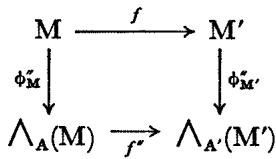
\includegraphics[keepaspectratio]{images/part003_899f4c21.jpg}}

and \(f''\) is a graded algebra homomorphism. It is immediately deduced that if \(\sigma: A' \to A''\) is another ring homomorphism, \(M''\) an \(A''\) -module, \(g: M' \to M''\) an \(A'\) -homomorphism (relative to \(\sigma\) ) and \(g'': \bigwedge_{A'}(M') \to \bigwedge_{A''}(M'')\) the corresponding \(A''\) -homomorphism of algebras, then the composite A-homomorphism of algebras

\[
\bigwedge_ {\mathbf {A}} (\mathbf {M}) \xrightarrow {f ^ {\prime \prime}} \bigwedge_ {\mathbf {A} ^ {\prime}} (\mathbf {M} ^ {\prime}) \xrightarrow {g ^ {\prime \prime}} \bigwedge_ {\mathbf {A} ^ {\prime \prime}} (\mathbf {M} ^ {\prime \prime})\tag{13}
\]

corresponds to the composite A-homomorphism \(g \circ f: \mathbf{M} \to \mathbf{M}''\) (relative to \(\sigma \circ \rho\) ).

PROPOSITION 8. Let A, B be two commutative rings, \(\rho: A \to B\) a ring homomorphism and M an A-module. The canonical extension

\[
\psi : \bigwedge_ {\mathbf {B}} (\mathbf {B} \otimes_ {\mathbf {A}} \mathbf {M}) \rightarrow \mathbf {B} \otimes_ {\mathbf {A}} \bigwedge_ {\mathbf {A}} (\mathbf {M})
\]

of the B-linear mapping \(l_{B} \otimes \phi_{M}^{\prime\prime}: B \otimes_{A} M \to B \otimes_{A} \bigwedge_{A}(M)\) is a graded B-algebra isomorphism.

The proof is derived from that of § 5, no. 4, Proposition 5 replacing T by \(\bigwedge\) and \(\phi_{\mathbf{M}}\) by \(\phi_{\mathbf{M}}^{\prime \prime}\) .

\subsection{DIRECT LIMITS OF EXTERIOR ALGEBRAS}

Let \((\mathbf{A}_{\alpha},\phi_{\beta \alpha})\) be a directed direct system of commutative rings, \((\mathbf{M}_{\alpha},f_{\beta \alpha})\) a direct system of \(\mathbf{A}_{\alpha}\) -modules, \(\mathbf{A} = \varinjlim \mathbf{A}_{\alpha}\) and \(\mathbf{M} = \varinjlim \mathbf{M}_{\alpha}\) . For \(\alpha \leqslant \beta\) , we derive canonically from the \(\mathbf{A}_{\alpha}\) -homomorphism \(f_{\beta \alpha}: \overrightarrow{\mathbf{M}_{\alpha}} \to \mathbf{M}_{\beta}\) an \(\mathbf{A}_{\alpha}\) -algebra homomorphism (no. 5, formula (12)) \(f_{\beta \alpha}^{\prime \prime}: \bigwedge_{\mathbf{A}_{\alpha}} (\mathbf{M}_{\alpha}) \to \bigwedge_{\mathbf{A}_{\beta}} (\mathbf{M}_{\beta})\) and it follows from (13) that \((\bigwedge_{\mathbf{A}_{\alpha}} (\mathbf{M}_{\alpha}), f_{\beta \alpha}^{\prime \prime})\) is a direct system of graded \(\mathbf{A}_{\alpha}\) -modules. On the other hand let \(f_{\alpha}: \mathbf{M}_{\alpha} \to \mathbf{M}\) be the canonical \(\mathbf{A}_{\alpha}\) -homomorphism; we derive (no. 5, formula (12)) a graded \(\mathbf{A}_{\alpha}\) -algebra homomorphism \(f_{\alpha}^{\prime \prime}: \bigwedge_{\mathbf{A}_{\alpha}} (\mathbf{M}_{\alpha}) \to \bigwedge_{\mathbf{A}} (\mathbf{M})\) and it also follows from (13) that the \(f_{\alpha}^{\prime \prime}\) constitute a direct system of \(\mathbf{A}_{\alpha}\) -homomorphisms.

PROPOSITION 9. The A-homomorphism \(f'' = \varinjlim f_{\alpha}' : \varinjlim \bigwedge_{A_{\alpha}}(M_{\alpha}) \to \bigwedge_{A}(M)\) is a graded algebra isomorphism.

The proof is the same as that of § 5, no. 4, Proposition 6 replacing throughout T by \(\bigwedge\) and \(\phi\) by \(\phi''\) and taking account of the fact that a direct limit of alternating algebras is alternating.

\subsection{EXTERIOR ALGEBRA OF A DIRECT SUM. EXTERIOR ALGEBRA OF A GRADED MODULE}

Let A be a commutative ring, \(M = \bigoplus_{\lambda \in L} M_{\lambda}\) the direct sum of a family of a family of A-modules and \(j_{\lambda}: M_{\lambda} \to M\) the canonical injection; an A-homomorphism of graded algebras \(\bigwedge(j_{\lambda}): \bigwedge(M_{\lambda}) \to \bigwedge(M)\) is derived. Since \(\bigwedge(M)\) is anticommutative, Proposition 10 of §4, no. 7 (or if need be generalized to the case where L is infinite, cf.~§4, no. 8, Remark 1) can be applied to the homomorphisms \(\bigwedge(j_{\lambda})\) ; then there exists a unique algebra homomorphism

\[
g \colon \bigotimes_ {\lambda \in L} ^ {g} \Lambda (M _ {\lambda}) \to \Lambda (M)\tag{14}
\]

(also denoted by \(g_{\mathbf{M}}\) ) such that \(\bigwedge (j_{\lambda}) = g \circ f_{\lambda}\) , where

\[
f _ {\lambda}: \bigwedge (\mathrm{M} _ {\lambda}) \rightarrow \bigotimes_ {\lambda \in L} ^ {g} \bigwedge (\mathrm{M} _ {\lambda})
\]

denotes the canonical homomorphism.

PROPOSITION 10. The canonical homomorphism \(g\) (formula (14)) is a graded algebra isomorphism.

To prove that \(g\) is bijective, we define a graded algebra homomorphism

\[
h: \bigwedge (\mathbf {M}) \rightarrow \bigotimes_ {\lambda \in L} ^ {\mathfrak {g}} \bigwedge (\mathbf {M} _ {\lambda})\tag{15}
\]

such that \(g \circ h\) and \(h \circ g\) are respectively the identity mappings on \(\bigwedge(\mathbf{M})\) and \(\bigotimes_{\lambda \in L} \bigwedge(\mathbf{M}_{\lambda})\) . For each \(\lambda \in L\) , consider the composite linear mapping

\[
u _ {\lambda}: \mathrm{M} _ {\lambda} \xrightarrow {\phi_ {\mathrm{M} _ {\lambda}} ^ {n}} \bigwedge (\mathrm{M} _ {\lambda}) \xrightarrow {f _ {\lambda}} \mathbf {g} _ {\lambda \in L} \bigotimes \bigwedge (\mathrm{M} _ {\lambda}).
\]

There exists one and only one A-linear mapping \(u: \mathbf{M} \to {}^{\mathfrak{g}} \bigotimes_{\lambda \in L} \bigwedge (\mathbf{M}_{\lambda})\) such that \(u \circ j_{\lambda} = u_{\lambda}\) for all \(\lambda \in L\) . The skew tensor product \({}^{\mathfrak{g}} \bigotimes_{\lambda \in L} \bigwedge (\mathbf{M}_{\lambda})\) is an alternating algebra: for, for L finite, this follows from § 4, no. 9, Proposition 14 and, for L arbitrary, this follows from the definition of this product given in § 4, no. 8, Remark 1 and the fact that a direct limit of alternating graded algebras is alternating. As also \(u(\mathbf{M})\) is contained in the submodule of elements of degree 1 in the graded algebra \(\bigotimes_{\lambda \in L} \bigwedge (\mathbf{M}_{\lambda})\) , it follows from no. 1, Proposition 1 and Remark 1 that there exists a unique graded algebra homomorphism.

\[
h: \bigwedge (\mathbf {M}) \rightarrow \bigotimes_ {\lambda \in L} ^ {\mathfrak {g}} \bigwedge (\mathbf {M} _ {\lambda})
\]

such that \(h \circ \phi_{\mathbf{M}}'' = u\) . The verification of the fact that \(g \circ h\) and \(h \circ g\) are the identity mappings is then performed as in §6, no. 6, Proposition 9 replacing \(\mathbf{S}\) by \(\bigwedge\) and \(\phi'\) by \(\phi''\) .

Remark. Let \(N = \bigoplus_{\lambda \in L} N_{\lambda}\) be the direct sum of another family of A-modules with L as indexing set and, for all \(\lambda \in L\) , let \(v_{\lambda}: M_{\lambda} \to N_{\lambda}\) be an A-linear mapping, whence there is an A-linear mapping \(v = \bigoplus_{\lambda} v_{\lambda}: M \to N\) (II, §1, no. 6, Proposition 7). Then the diagram

\[
\begin{array}{c c c} \mathbf {g} _ {\lambda \in L} ^ {\otimes} \wedge (\mathrm{M} _ {\lambda}) & \xrightarrow {g _ {\mathrm{M}}} & \wedge (\mathrm{M}) \\ \bigotimes_ {\lambda \in L} \wedge (v _ {\lambda}) \Big \downarrow & & \Big \downarrow \wedge (v) \\ \mathbf {g} _ {\lambda \in L} ^ {\otimes} \wedge (\mathrm{N} _ {\lambda}) & \xrightarrow {g _ {\mathrm{N}}} & \wedge (\mathrm{N}) \end{array}
\]

is commutative (cf.~§ 4, no. 5, Corollary to Proposition 8).

The sub-A-module of \(\mathbf{g}_{\lambda \in L}^{\otimes} \bigwedge (\mathbf{M}_{\lambda})\) with which \(\bigwedge^{n}(\mathbf{M})\) is identified by means of the isomorphism \(g\) can be described more precisely. For every finite subset \(J\) of \(L\) , we write \(\mathrm{E}_{J} = \mathbf{g}_{\lambda \in J}^{\otimes} \bigwedge (\mathbf{M}_{\lambda})\) , so that \(\mathbf{g}_{\lambda \in L}^{\otimes} \bigwedge (\mathbf{M}_{\lambda}) = \lim_{\lambda \to 0} \mathrm{E}_{J}\) relative to the directed set \(\mathfrak{F}(L)\) of finite subsets of \(L\) , by definition (§ 4, no. 8, Remark 1). For every family \(\nu = (n_{\lambda}) \in \mathbf{N}^{(L)}\) (therefore with finite support) such that \(\sum_{\lambda \in L} n_{\lambda} = n\) and every finite subset \(J\) of \(L\) containing the support of the family \(\nu\) , we write

\[
\bigwedge^ {J, v} (\mathbf {M}) = \bigotimes_ {\lambda \in J} \bigwedge^ {n _ {\lambda}} (\mathbf {M} _ {\lambda})\tag{16}
\]

so that the submodule \(\mathbf{E}_{\mathbf{J},n}\) of elements of degree \(n\) in \(\mathbf{E}_{\mathbf{J}}\) is the direct sum of the \(\bigwedge^{\mathbf{J},\nu}(\mathbf{M})\) for all families \(\nu\) of support contained in \(\mathbf{J}\) and such that

\[
\sum_ {\lambda \in L} n _ {\lambda} = n
\]

(§ 4, no. 7, Proposition 10 and no. 8). By way of convention we write \(\bigwedge^{J,\nu}(\mathbf{M}) = \{0\}\) for the families \(\nu\) whose support is not contained in \(J\) ; then

\(E_{J,n}\) can also be called the direct sum of all the \(\bigwedge^{J,\nu}(M)\) , where \(\nu\) runs through the set \(H_n\) of all families \(\nu = (n_\lambda)_{\lambda \in L}\) such that \(\sum_{\lambda \in L} n_\lambda = n\) . Since \(\bigwedge^0(M_\lambda)\) is identified with A, clearly also for two finite subsets \(J \subset J'\) of L and a family \(\nu\) of support contained in J, the canonical mapping \(\bigwedge^{J,\nu}(M) \to \bigwedge^{J',\nu}(M)\) (restriction of the canonical mapping \(E_J \to E_{J'}\) to \(\bigwedge^{J,\nu}(M)\) ) is bijective. If we write, for all \(\nu \in H_n\) ,

\[
\bigwedge^ {\nu} (\mathbf {M}) = \varinjlim \bigwedge^ {J, \nu} (\mathbf {M})\tag{17}
\]

it is then seen that, taking account of II, § 6, no. 2, Proposition 5, we have:

COROLLARY. The A-module \(\bigwedge^{n}(\mathbf{M})\) is the image under isomorphism (14) of the submodule of \(\bigotimes_{\lambda \in L} \bigwedge (\mathbf{M}_{\lambda})\) the direct sum of the submodules \(\bigwedge^{\nu}(\mathbf{M})\) for all families \(\nu = (n_{\lambda}) \in \mathbf{N}^{(L)}\) such that \(\sum_{\lambda \in L} n_{\lambda} = n\) ; if \(J\) is the support of \(\nu, \bigwedge^{\nu}(\mathbf{M})\) is canonically isomorphic to \(\bigotimes_{\lambda \in J} \bigwedge^{n_{\lambda}}(\mathbf{M}_{\lambda})\) .

In general \(\bigwedge^{\nu}(\mathbf{M}),\bigotimes_{\lambda \in J}\bigwedge^{n_{\lambda}}(\mathbf{M}_{\lambda})\) and their image in \(\bigwedge^n (\mathbf{M})\) are identified. With this convention:

PROPOSITION 11. Let \(\Delta\) be a commutative monoid, \(\mathbf{M}\) a graded A-module of type \(\Delta\) and \((\mathbf{M}_{\alpha})_{\alpha \in \Delta}\) its graduation. For every ordered pair \((\alpha, n) \in \Delta \times \mathbf{N}\) , let \(\bigwedge^{\alpha, n}(\mathbf{M})\) be the submodule of \(\bigwedge^n (\mathbf{M})\) the direct sum of the submodules \(\bigotimes_{\lambda \in J} \bigwedge^{n_{\lambda}}(\mathbf{M}_{\alpha_{\lambda}})\) , where \((n_{\lambda})_{\lambda \in L}\) runs through the set of families of integers \(\geqslant 0\) such that \(\sum_{\lambda \in L} n_{\lambda} = n\) , \(J\) is its support and, for each \((n_{\lambda})\) , \((\alpha_{\lambda})_{\lambda \in J}\) runs through the set of families of \(\Delta^J\) such that \(\sum_{\lambda \in J} \alpha_{\lambda} = \alpha\) . Then \((\bigwedge^{\alpha, n}(\mathbf{M}))_{(\alpha, n) \in \Delta \times N}\) is the only graduation of type \(\Delta \times N\) compatible with the algebra structure on \(\bigwedge(\mathbf{M})\) and which induces on \(\mathbf{M} = \bigwedge^1 (\mathbf{M})\) the given graduation.

The fact that \(\bigwedge (\mathbf{M})\) is the direct sum of the \(\bigwedge^{\alpha ,n}(\mathbf{M})\) follows from the Corollary to Proposition 10; the rest of the proof is identical with the end of the proof of §5, no. 5, Proposition 7.

\subsection{EXTERIOR ALGEBRA OF A FREE MODULE}

THEOREM 1. Let M be an A-module with a basis \((e_{\lambda})_{\lambda \in L}\) . Let L be given the structure of a totally ordered set (Set Theory, III, §2, no. 3, Theorem 1) and for every finite subset J of L we write

\[
e _ {J} = e _ {\lambda_ {1}} \wedge e _ {\lambda_ {2}} \wedge \dots \wedge e _ {\lambda_ {n}}\tag{18}
\]

where \((\lambda_k)_{1 \leqslant k \leqslant n}\) is the sequence of elements of \(J\) arranged in increasing order (Set Theory, III, § 5, no. 3, Proposition 6); we write \(e_\varphi = 1\) , the unit element of A. Then the \(e_J\) , where \(J\) runs through the set \(\mathfrak{F}(L)\) of finite subsets of \(L\) , form a basis of the exterior algebra \(\bigwedge(M)\) .

Since the \(e_{\lambda}\) generate the A-module M, every element of \(\bigwedge(\mathbf{M})\) is a linear combination of a finite number of products of the elements \(e_{\lambda}\) and hence (taking account of no. 3, Proposition 5) is a linear combination of a finite number of elements \(e_{J}\) for \(J \in \mathfrak{F}(L)\) . It reduces to proving that the \(e_{J}\) are linearly independent over A. Otherwise, there would exist between these elements a linear relation with coefficients not all zero; the union of the subsets J which correspond to the \(e_{J}\) whose coefficients in this relation are \(\neq 0\) is a finite subset K of L (since there is only a finite number of coefficients \(\neq 0\) ). Let N be the submodule of M generated by the \(e_{\lambda}\) such that \(\lambda \in K\) ; N is a direct factor in M, hence (no. 2) \(\bigwedge(\mathbf{N})\) is identified with a subalgebra of \(\bigwedge(\mathbf{M})\) and, if we show that the \(e_{J}\) with \(J \subset K\) form a basis of \(\bigwedge(\mathbf{N})\) , we shall obtain the desired contradiction.

It therefore reduces to providing Theorem 1 when the basis of M is finite; we may therefore suppose that \(L = [1, m] \subset N\) . For each \(i \in L\) , let \(M_i\) be the free submodule \(Ae_i\) of M; M is the direct sum of the \(M_i\) and \(\bigwedge(M_i)\) is the direct sum of \(\bigwedge^0(M_i) = A\) and \(\bigwedge^1(M_i) = M_i\) (no. 3, Proposition 6). Let \(\bigwedge(M)\) be canonically identified with the A-module the tensor product of the \(\bigwedge(M_i)\) (no. 7, Proposition 10); the latter has as basis the tensor product of the bases \((1, e_i)\) of the \(\bigwedge(M_i)\) (II, § 3, no. 7, Corollary 2 to Proposition 7); thus we obtain all the elements

\[
u _ {1} \otimes u _ {2} \otimes \dots \otimes u _ {m}
\]

where either \(u_{i}=1\) or \(u_{i}=e_{i}\) ; if J is the set of indices i such that \(u_{i}=e_{i}\) , \(u_{1}\otimes u_{2}\otimes\cdots\otimes u_{m}\) is identical with \(e_{J}\) , which completes the proof.

COROLLARY 1. Suppose that \(\mathbf{L} = [1, m]\) ; then the basis \((e_{\mathrm{J}})_{\mathrm{J} \in \mathfrak{P}(\mathrm{L})}\) of \(\bigwedge (\mathbf{M})\) has \(2^{m}\) elements. For \(p > m\) , \(\bigwedge^{p}(\mathbf{M}) = \{0\}\) ; \(\bigwedge^{m}(\mathbf{M})\) has a basis consisting of a single element \(e_{\mathrm{L}}\) ; for \(0 \leqslant p \leqslant m\) the number of elements in the basis \((e_{\mathrm{J}})\) of \(\bigwedge^{p}(\mathbf{M})\) consisting of the \(e_{\mathrm{J}}\) such that \(\operatorname{Card}(\mathbf{J}) = p\) is

\[
\binom {m} {p} = \frac {m !}{p ! (m - p) !}.
\]

This follows from Set Theory, III, § 3, no. 5, Proposition 12 and Set Theory, III, § 5, no. 8, Corollary 1 to Proposition 11.

We return to the case where the set L in Theorem 1 is arbitrary and give explicitly the multiplication table (§ 1, no. 7) of the basis \((e_{J})\) . Given two finite subsets \(J\) , \(K\) of the totally ordered set \(L\) , we write

\[
\left\{ \begin{array}{l l} \rho_ {J, K} = 0 & \text { if } J \cap K \neq \varnothing \\ \rho_ {J, K} = (- 1) ^ {\nu} & \text { if } J \cap K = \varnothing \end{array} \right.\tag{19}
\]

where v denotes the number of ordered pairs \((\lambda, \mu) \in J \times K\) such that \(\lambda > \mu\) . Then Corollary 1 to Proposition 4 of no. 2 immediately implies the relation

\[
e _ {J} \wedge e _ {K} = \rho_ {J, K} e _ {J \cup K}.\tag{20}
\]

Note the formula

\[
\rho_ {J, K} \rho_ {K, J} = (- 1) ^ {j k}\tag{21}
\]

when \(\mathbf{J} \cap \mathbf{K} = \varnothing, j = \operatorname{Card}(\mathbf{J}), k = \operatorname{Card}(\mathbf{K})\) (no. 3, Corollary 2 to Proposition 5.)

COROLLARY 2. If M is a projective A-module, \(\bigwedge (\mathbf{M})\) is a projective A-module.

The proof is the same as that of § 5, no. 5, Corollary to Theorem 1 replacing T by \(\Lambda\) .

COROLLARY 3. Let M be a projective A-module and \((x_{i})_{1\leqslant i\leqslant n}\) a finite sequence of elements of M. For there to exist on M an alternating \(n\) -linear form \(f\) such that

\[
f (x _ {1}, x _ {2}, \dots , x _ {n}) \neq 0,
\]

it is necessary and sufficient that \(x_{1} \wedge x_{2} \wedge \cdots \wedge x_{n} \neq 0\) .

We know already (with no hypothesis on M) that the condition is necessary (no. 4, Proposition 7). Suppose now that M is projective and that

\[
x _ {1} \wedge x _ {2} \wedge \dots \wedge x _ {n} \neq 0.
\]

Then \(\bigwedge^n (\mathbf{M})\) is projective (Corollary 2) and hence the canonical mapping

\[
\bigwedge^ {n} (\mathbf {M}) \rightarrow (\bigwedge^ {n} (\mathbf {M})) ^ {* *}
\]

is injective (II, §2, no. 7, Corollary 4 to Proposition 13); we conclude that there exists a linear form \(g: \bigwedge^{n}(\mathbf{M}) \to \mathbf{A}\) such that \(g(x_{1} \wedge x_{2} \wedge \dots \wedge x_{n}) \neq 0\) . If \(f\) is the alternating \(n\) -linear form corresponding to \(g\) (no. 4, Proposition 7), then \(f(x_{1}, \ldots, x_{n}) \neq 0\) .

\subsection{CRITERIA FOR LINEAR INDEPENDENCE}

PROPOSITION 12. Let M be a projective A-module. For elements \(x_1, x_2, \ldots, x_n\) of M to be linearly dependent, it is necessary and sufficient that there exist \(\lambda \neq 0\) in A such that

\[
\lambda x _ {1} \wedge x _ {2} \wedge \dots \wedge x _ {n} = 0.\tag{22}
\]

The condition is necessary (with no hypothesis on M), for if for example \(\lambda x_{1}\) (with \(\lambda \neq 0\) ) is a linear combination of \(x_{2}, \ldots, x_{n}\) , relation (22) holds (no. 3, Proposition 5). We show that the condition is sufficient by induction on n; for n = 1, it is a trivial consequence of the definition. Suppose therefore that n \textgreater{} 1 and that condition (22) holds for some \(\lambda \neq 0\) . If

\[
\lambda x _ {2} \wedge x _ {3} \wedge \dots \wedge x _ {n} = 0,
\]

then the induction hypothesis implies that \(x_{2},\ldots,x_{n}\) are linearly dependent and hence a fortiori \(x_{1},x_{2},\ldots,x_{n}\) are. If \(\lambda x_{2}\wedge x_{3}\wedge\cdots\wedge x_{n}\neq0\) , it follows from no. 8, Corollary 3 to Theorem 1 that there exists an alternating \((n-1)\) -linear form f such that \(f(\lambda x_{2}\wedge x_{3}\wedge\cdots\wedge x_{n})=\mu\neq0\) . Since

\[
x _ {1} \wedge (\lambda x _ {2}) \wedge \dots \wedge x _ {n} = 0,
\]

it follows from no. 8, Corollary 3 to Theorem 1 that \(\mu x_{1}\) is a linear combination of \(\lambda x_{2}, x_{3}, \ldots, x_{n}\) ; hence \(x_{1}, x_{2}, \ldots, x_{n}\) are linearly dependent.

COROLLARY. Let M and N be two projective A-modules and \(f:M\to N\) an A-linear mapping. If f is injective, then \(\bigwedge(f):\bigwedge(\mathbf{M})\to\bigwedge(\mathbf{N})\) is injective.

We prove this first under the assumption that M is free; let \((e_{\lambda})_{\lambda \in L}\) be a basis of M, so that \((e_{J})_{J \in \mathfrak{F}(L)}\) (formula (18)) is a basis of \(\bigwedge(M)\) . Suppose that the kernel of \(\bigwedge(f)\) contains an element \(u = \sum_{J} \alpha_{J} e_{J} \neq 0\) . Let K be an element minimal among the finite subsets J such that \(\alpha_{J} \neq 0\) and let H be a finite subset of L disjoint from K and such that \(K \cup H\) contains all the J (finite in number) such that \(\alpha_{J} \neq 0\) ; for all \(J \neq K\) such that \(\alpha_{J} \neq 0\) , we have therefore by definition \(J \cap H \neq 0\) and consequently (no. 8, formula (20)).

\[
u \wedge e _ {\mathrm{H}} = + \alpha_ {\mathbf {K}} e _ {\mathbf {K} \cup \mathbf {H}}
\]

belongs to the two-sided ideal of \(\bigwedge (\mathbf{M})\) , the kernel of \(\bigwedge (f)\) . We write \(e_{\mathbf{K} \cup \mathbf{H}} = e_{\lambda_1} \wedge e_{\lambda_2} \wedge \dots \wedge e_{\lambda_n}\) ; then \(\alpha_{\mathbf{K}} f(e_{\lambda_1}) \wedge f(e_{\lambda_2}) \wedge \dots \wedge f(e_{\lambda_n}) = 0\) ; by virtue of Proposition 12, the elements \(f(e_{\lambda_i})\) ( \(1 \leqslant i \leqslant n\) ) of N are linearly dependent. But this contradicts the hypothesis that \(f\) is injective (II, §1, no. 11, Corollary 3 to Proposition 17).

We now consider the general case; let \(\mathbf{M}'\) be an A-module such that \(\mathbf{M} \oplus \mathbf{M}' = \mathbf{P}\) is free (II, § 2, no. 2, Proposition 4). Consider the linear mapping \(g: \mathbf{M} \oplus \mathbf{M}' \to \mathbf{N} \oplus \mathbf{M} \oplus \mathbf{M}'\) such that \(g(x, y) = (f(x), 0, y)\) , so that there is a commutative diagram

\pandocbounded{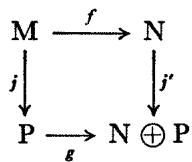
\includegraphics[keepaspectratio]{images/part004_a147f11a.jpg}}

where the vertical arrows are the canonical injections. Since g is injective and P is free, \(\bigwedge(g)\) is an injective homomorphism as has been seen above. Now, \(\bigwedge(j):\bigwedge(\mathbf{M})\to\bigwedge(\mathbf{P})\) is an injective homomorphism since M is a direct factor in P (no. 2). The composite homomorphism

\[
\bigwedge (\mathbf {M}) \xrightarrow {\bigwedge (j)} \bigwedge (\mathbf {P}) \xrightarrow {\bigwedge (g)} \bigwedge (\mathbf {N} \oplus \mathbf {P})
\]

is therefore injective and, as it is also equal to the composite homomorphism

\[
\Lambda (\mathbf {M}) \xrightarrow {\Lambda (f)} \Lambda (\mathbf {N}) \xrightarrow {\Lambda (j ^ {\prime})} \Lambda (\mathbf {N} \oplus \mathbf {P})
\]

we conclude that \(\bigwedge (f)\) is injective.

PROPOSITION 13. Let M be an A-module, N a direct factor submodule of M which is free of dimension p and \(\{u\}\) a basis of \(\bigwedge^{p}(\mathbf{N})\) . For an element \(x \in M\) to belong to N, it is necessary and sufficient that \(u \wedge x = 0\) .

Let P be a submodule of M complementary to N and let \(y \in N\) , \(z \in P\) be such that \(x = y + z\) . Then \(u \wedge x = u \wedge z\) . As \(\bigwedge^{p}(N)\) is free of dimension 1, the mapping \(\phi: P \to P \otimes \bigwedge^{p}(N)\) such that \(\phi(p) = p \otimes u\) is bijective (II, §3, no. 4, Proposition 4). On the other hand (no. 7, Proposition 10), the composition of the canonical homomorphisms

\[
\psi : \mathrm{P} \otimes \bigwedge^ {p} (\mathrm{N}) \rightarrow \bigwedge (\mathrm{P}) \otimes \bigwedge (\mathrm{N}) \rightarrow \bigwedge (\mathrm{M})
\]

is injective. The mapping \(\psi \circ \phi\) is therefore injective, whence the proposition.

THEOREM 2. Let \(\mathbf{M}\) be an A-module with a finite basis \((e_i)_{1\leqslant i\leqslant n}\) . For a sequence \((x_i)_{1\leqslant i\leqslant n}\) of \(n\) elements of \(\mathbf{M}\) to form a basis of \(\mathbf{M}\) , it is necessary and sufficient that the element \(\lambda \in \mathbf{A}\) such that

\[
x _ {1} \wedge x _ {2} \wedge \dots \wedge x _ {n} = \lambda . e _ {1} \wedge e _ {2} \wedge \dots \wedge e _ {n}\tag{23}
\]

be invertible in A.

Recall that \(e_{1} \wedge e_{2} \wedge \cdots \wedge e_{n}\) is the unique element of a basis of \(\bigwedge^{n}(\mathbf{M})\) (no. 8, Corollary 1 to Theorem 1) so that the element \(\lambda \in A\) satisfying (23) is determined uniquely. If \((x_{i})_{1 \leqslant i \leqslant n}\) is a basis of M, \(x_{1} \wedge x_{2} \wedge \cdots \wedge x_{n}\) is the unique element in a basis of \(\bigwedge^{n}(\mathbf{M})\) (no. 8), then \(\lambda\) is invertible. Conversely, suppose \(\lambda\) is invertible; then the alternating n-linear form f corresponding to the linear mapping \(g: \bigwedge^{n}(\mathbf{M}) \to \mathbf{A}\) such that

\[
g (e _ {1} \wedge e _ {2} \wedge \dots \wedge e _ {n}) = \lambda^ {- 1}
\]

is such that \(f(x_{1}, x_{2}, \ldots, x_{n}) = 1\) . For all \(x \in \mathbf{M}\) , obviously

\[
x \wedge x _ {1} \wedge \dots \wedge x _ {n} = 0
\]

(no. 3, Proposition 6); applying no. 8, Corollary 3 to Theorem 1, we obtain

\[
f (x _ {1}, x _ {2}, \dots , x _ {n}). x = \sum_ {i = 1} (- 1) ^ {i - 1} f (x, x _ {1}, \dots , \hat {x} _ {i}, \dots , x _ {n}). x _ {i}.
\]

As \(f(x_{1},\ldots ,x_{n}) = 1\) , this shows that every \(x\in \mathbf{M}\) is a linear combination of \(x_{1},x_{2},\ldots ,x_{n}\) and, as the latter are linearly independent (since

\[
x _ {1} \wedge x _ {2} \wedge \dots \wedge x _ {n} \neq 0),
\]

they form a basis of M.

\section{DETERMINANTS}

\subsection{DETERMINANTS OF AN ENDOMORPHISM}

Let M be an A-module with a finite basis of n elements and u an endomorphism of M. The A-module \(\bigwedge^{n}(\mathbf{M})\) is a monogenous free module, that is isomorphic to A (no. 8, Corollary 1 to Theorem 1); \(\bigwedge^{n}(u)\) is an endomorphism of this module and is therefore a homothety \(z \mapsto \lambda z\) of ratio \(\lambda \in A\) determined uniquely (II, §2, no. 3, Proposition 5).

DEFINITION 1. The determinant of an endomorphism \(u\) of a free A-module \(M\) of finite dimension \(n\) (II, §7, no. 2, Corollary to Proposition 3 and Remark 1), denoted by \(\det u\) , is the scalar \(\lambda\) such that \(\bigwedge^{n}(u)\) is the homothety of ratio \(\lambda\) .

By formula (4) of §7, no. 2, det u is the unique scalar such that

\[
u \left(x _ {1}\right) \wedge u \left(x _ {2}\right) \wedge \dots \wedge u \left(x _ {n}\right) = (\det u). x _ {1} \wedge x _ {2} \wedge \dots \wedge x _ {n}\tag{1}
\]

for every sequence \((x_{i})_{1\leqslant i\leqslant n}\) of \(n\) elements of M. If \(\det (u) = 1\) , \(u\) is said to be unimodular.

PROPOSITION 1. (i) If \(u\) and \(v\) are two endomorphisms of a finite-dimensional free A-module M, then

\[
\det (u \circ v) = (\det u) (\det v).\tag{2}
\]

\begin{enumerate}
\def\labelenumi{(\roman{enumi})}
\setcounter{enumi}{1}
\tightlist
\item
  \(\operatorname{det}(1_{\mathbf{M}}) = 1\) ; for every automorphism \(u\) of \(\mathbf{M}\) , \(\operatorname{det} u\) is invertible in \(\mathbf{A}\) and
\end{enumerate}

\[
\det (u ^ {- 1}) = (\det u) ^ {- 1}.\tag{3}
\]

If \(n\) is the dimension of \(\mathbf{M}\) , this follows immediately from the relation \(\bigwedge^{n}(u \circ v) = (\bigwedge^{n}(u)) \circ (\bigwedge^{n}(v))\) (§ 7, no. 2, formula (3)).

Let M be a free A-module with a finite basis \((e_{i})_{1\leqslant i\leqslant n}\) ; given a sequence \((x_{i})_{1\leqslant i\leqslant n}\) of n elements of M, the determinant of this sequence with respect to the given basis \((e_i)\) , denoted by \(\det(x_1, x_2, \ldots, x_n)\) when no confusion can arise over the basis, is the determinant of the endomorphism \(u\) of M such that \(u(e_i) = x_i\) for \(1 \leqslant i \leqslant n\) . Then by formula (1)

\[
x _ {1} \wedge x _ {2} \wedge \dots \wedge x _ {n} = \det (x _ {1}, x _ {2}, \dots , x _ {n}) e _ {1} \wedge e _ {2} \wedge \dots \wedge e _ {n}\tag{4}
\]

and this relation characterizes the mapping \((x_{i})\mapsto\det(x_{1},x_{2},\ldots,x_{n})\) of \(\mathbf{M}^{n}\) into A. It shows that this mapping is an alternating \(n\) -linear form. As, by virtue of §7, no. 4, Proposition 7, the A-module of alternating \(n\) -linear forms is canonically isomorphic to the dual of \(\bigwedge^{n}(\mathbf{M})\) and \(\bigwedge^{n}(\mathbf{M})\) is isomorphic to A, it is seen that every alternating \(n\) -linear form on \(\mathbf{M}^{n}\) can be written

\[
(x _ {1}, \dots , x _ {n}) \mapsto \alpha \det (x _ {1}, x _ {2}, \dots , x _ {n})
\]

for some \(\alpha \in \mathbf{A}\) .

PROPOSITION 2. Let M be a free A-module with a finite basis \((e_i)_{1 \leqslant i \leqslant n}\) and \(v\) an endomorphism of M. For every sequence \((x_i)_{1 \leqslant i \leqslant n}\) of \(n\) elements of M,

\[
\det (v (x _ {1}), \dots , v (x _ {n})) = (\det v) \det (x _ {1}, \dots , x _ {n}).\tag{5}
\]

If \(u\) is the endomorphism of \(M\) such that \(u(e_i) = x_i\) for all \(i\) , then

\[
v (x _ {i}) = (v \circ u) (e _ {i})
\]

and (5) therefore follows from (2).

\subsection{CHARACTERIZATION OF AUTOMORPHISMS OF A FINITE-DIMENSIONAL FREE MODULE}

THEOREM 1. Let M be a finite-dimensional free A-module and u an endomorphism of M. The following conditions are equivalent:

\begin{enumerate}
\def\labelenumi{(\alph{enumi})}
\item
  u is bijective;
\item
  \(u\) is right invertible (II, § 1, no. 9, Corollary 1 to Proposition 15);
\item
  u is left invertible (II, § 1, no. 9, Corollary 2 to Proposition 15);
\item
  u is surjective;
\item
  det u is invertible in A.
\end{enumerate}

Let \((e_i)_{1\leqslant i\leqslant n}\) be a basis of M. If \(x_{i} = u(e_{i})\) for \(1\leqslant i\leqslant n\) , then

\[
x _ {1} \wedge x _ {2} \wedge \dots \wedge x _ {n} = (\det u) e _ {1} \wedge e _ {2} \wedge \dots \wedge e _ {n}.
\]

By § 7, no. 9, Theorem 2 a necessary and sufficient condition for the \(x_{i}\) to form a basis of M is that \(\det u\) be an invertible element of A; this proves the equivalence of (a) and (e). Observe that (a) obviously implies each of conditions (b), (c) and (d); it remains to prove that each of conditions (b), (c) and (d) implies (e). Now, if there exists an endomorphism \(v\) of M such that \(v \circ u = 1_{\mathbf{M}}\) or \(u \circ v = 1_{\mathbf{M}}\) , then \((\det v)(\det u) = 1\) and hence \(\det u\) is invertible in A. If \(u\) is surjective, so is \(\bigwedge^{n}(u)\) ( \(\S 7\) , no. 2, Proposition 3), in other words the homothety of ratio det \(u\) in A is surjective, which immediately implies that det \(u\) is invertible.

PROPOSITION 3. Let M be a finite-dimensional free A-module. For every endomorphism u of M, the following conditions are equivalent:

\begin{enumerate}
\def\labelenumi{(\alph{enumi})}
\setcounter{enumi}{5}
\item
  u is injective;
\item
  det u is not a divisor of zero in A.
\end{enumerate}

With the same notation as in the proof of Theorem 1, for u to be injective, it is necessary and sufficient that the \(x_{i}\) be linearly independent. By §7, no. 9, Proposition 12, it is necessary and sufficient for this that the relation \(\lambda x_{1} \wedge x_{2} \wedge \cdots \wedge x_{n} = 0\) (with \(\lambda \in A\) ) imply \(\lambda = 0\) . But this is equivalent to \(\lambda(\det u) = 0\) since \(e_{1} \wedge \cdots \wedge e_{n}\) is a basis of \(\bigwedge^{n}(M)\) ; whence the proposition.

Remark. When A is a field, condition (e) of Theorem 2 is equivalent to condition (g) of Proposition 3, since they both mean that det \(u \neq 0\) . In this case therefore all the conditions of Theorem 1 and Proposition 3 are equivalent (cf.~II, §7, no. 4, Corollary to Proposition 9).

\subsection{DETERMINANT OF A SQUARE MATRIX}

DEFINITION 2. Let I be a finite set, A a commutative ring and X a square matrix of type (I, I) over the ring A (II, § 10, no. 7). The determinant of the endomorphism u of the A-module A \(^{I}\) , whose matrix with respect to the canonical basis of A \(^{I}\) is X, is called the determinant of X and denoted by det X.

If \(X = (\xi_{ij})_{(i,j) \in I \times I}\) and \((e_i)_{i \in I}\) is the canonical basis of \(A^I\) , the endomorphism \(u\) is then given by

\[
u (e _ {i}) = \sum_ {j \in J} \xi_ {j i} e _ {j}.
\]

When \(\mathbf{I} = [1, n] \subset \mathbf{N}\) , if we write \(x_{i} = u(e_{i})\) for \(i \in \mathbf{I}\) , the determinant of \(X\) is then defined in the relation

\[
x _ {1} \wedge x _ {2} \wedge \dots \wedge x _ {n} = (\det X) e _ {1} \wedge e _ {2} \wedge \dots \wedge e _ {n}\tag{6}
\]

in other words, det X is equal to the determinant \(\det(x_{1}, x_{2}, \ldots, x_{n})\) with respect to the canonical basis of \(A^{n}\) . Consequently:

PROPOSITION 4. For \(n\) vectors \(x_1, \ldots, x_n\) of \(A^n\) , let \(X(x_1, \ldots, x_n)\) denote the square matrix of order \(n\) whose \(i\) -th column is \(x_i\) for \(1 \leqslant i \leqslant n\) . Then the mapping

\[
(x _ {1}, \dots , x _ {n}) \mapsto \det (X (x _ {1}, \dots , x _ {n}))
\]

of \((\mathbf{A}^n)^n\) into \(\mathbf{A}\) is alternating and \(n\) -linear.

In particular, the determinant of a matrix two of whose columns are equal is zero. If a permutation is performed on the columns of a matrix, the determinant of the new matrix is equal to that of the old multiplied by \(\varepsilon_{\sigma}\) . If to one column of a matrix is added a scalar multiple of a column of a different index, the determinant of the new matrix is equal to that of the old.

More generally, let M be a free A-module of finite dimension n and let \((e_{i})_{i\in I}\) be a basis of M; for every automorphism u of M, if X is the matrix of u with respect to the basis \((e_{i})\) , then

\[
\det (u) = \det (X)\tag{7}
\]

as follows immediately from the definitions.

When \(\mathbf{I} = [1, n]\) , the determinant of \(X\) is also denoted by

\[
\det (\xi_ {i j}) _ {1 \leqslant i \leqslant n, 1 \leqslant j \leqslant n}
\]

or simply \(\operatorname{det}(\xi_{ij})\) if this causes no confusion, or also

\[
\left| \begin{array}{c c c c c} \xi_ {1 1} & \xi_ {1 2} & \ldots & \xi_ {1 n} \\ \xi_ {2 1} & \xi_ {2 2} & \ldots & \xi_ {2 n} \\ \cdot & \cdot & \cdot & \cdot & \cdot \\ \xi_ {n 1} & \xi_ {n 2} & \ldots & \xi_ {n n} \end{array} \right|
\]

When \(X = 1\) , the matrix \(X\) is called unimodular.

Examples. (1) The determinant of the empty matrix is equal to 1; the determinant of a square matrix of order 1 is equal to the unique element of this matrix. For a matrix of order 2

\[
\left( \begin{array}{c c} \xi_ {1 1} & \xi_ {1 2} \\ \xi_ {2 1} & \xi_ {2 2} \end{array} \right)
\]

then, in the above notation,

\[
x _ {1} \wedge x _ {2} = (\xi_ {1 1} e _ {1} + \xi_ {2 1} e _ {2}) \wedge (\xi_ {1 2} e _ {1} + \xi_ {2 2} e _ {2}) = \xi_ {1 1} \xi_ {2 2} e _ {1} ^ {\prime} \wedge e _ {2} + \xi_ {2 1} \xi_ {1 2} e _ {2} \wedge e _ {1}
\]

whence

\[
\left| \begin{array}{c c} \xi_ {1 1} & \xi_ {1 2} \\ \xi_ {2 1} & \xi_ {2 2} \end{array} \right| = \xi_ {1 1} \xi_ {2 2} - \xi_ {1 2} \xi_ {2 1}.
\]

We translate into the language of matrices some of the results of nos. 1 and 2:

PROPOSITION 5. If X and Y are two square matrices over a commutative ring A with the same finite indexing set, then

\[
\det (X Y) = (\det X) (\det Y).\tag{8}
\]

For \(X\) to be invertible, it is necessary and sufficient that \(\det X\) be an invertible element of \(\mathbf{A}\) , and then

\[
\det (X ^ {- 1}) = (\det X) ^ {- 1}.\tag{9}
\]

This follows immediately from no. 1, Proposition 1 and no. 2, Theorem 1.

COROLLARY. Two similar square matrices have equal determinants.

If \(P\) is an invertible square matrix, then \(\det(PXP^{-1}) = \det X\) by (8) and (9).

PROPOSITION 6. For the columns of a square matrix X of finite order to be linearly independent, it is necessary and sufficient that det X be not a divisor of zero in A.

This follows from no. 2, Proposition 3.

\subsection{CALCULATION OF A DETERMINANT}

Lemma 1. Let A be a commutative ring and M a free A-module with a basis \((e_j)_{j \in J}\) , where the indexing set \(J\) is totally ordered. For every integer \(p \leqslant \operatorname{Card}(J)\) , every alternating \(p\) -linear function \(f: \mathbf{M}^p \to \mathbf{N}\) (where \(N\) is an A-module) and every family of \(p\) elements \(x_i = \sum_{j \in J} \xi_{ji} e_j\) of \(M\) ( \(1 \leqslant i \leqslant p\) ),

\[
\begin{array}{r l} f (x _ {1}, x _ {2}, \dots , x _ {p}) & = \sum_ {j _ {1} <   j _ {2} <   \dots <   j _ {p}} \left(\sum_ {\sigma \in \mathfrak {S} _ {p}} \varepsilon_ {\sigma}. \xi_ {j _ {\sigma (1)}, 1} \xi_ {j _ {\sigma (2)}, 2} \dots \xi_ {j _ {\sigma (p)}, p}\right) f (e _ {j _ {1}}, \dots , e _ {j _ {p}}) \end{array}\tag{10}
\]

where \((j_k)_{1\leqslant k\leqslant p}\) runs through the set of strictly increasing sequences of \(p\) elements of J.

Now

\[
f (x _ {1}, \dots , x _ {p}) = \sum_ {(j _ {k})} \xi_ {j _ {1}, 1} \xi_ {j _ {2}, 2} \dots \xi_ {j _ {p}, p} f (e _ {j _ {1}}, e _ {j _ {2}}, \dots , e _ {j _ {p}})
\]

where \((j_k)_{1 \leqslant k \leqslant p}\) runs through all the sequences of \(p\) elements of \(J\) ; it then suffices to apply Corollary 1 to Proposition 7 of §7, no. 4 to \(f\) .

In particular, if J is finite and has n elements and \(x_{i} = \sum_{j \in J} \xi_{ji} e_{j} (1 \leqslant i \leqslant n)\) are n elements of M, then

\[
\begin{array}{l} \text {(11)} \quad x _ {1} \wedge x _ {2} \wedge \dots \wedge x _ {n} \\ = \left(\sum_ {\sigma \in \mathfrak {S} _ {n}} \varepsilon_ {\sigma} \xi_ {j _ {\sigma (1)}, 1} \xi_ {j _ {\sigma (2)}, 2} \dots \xi_ {j _ {\sigma (n)}, n}\right) e _ {j _ {1}} \wedge e _ {j _ {2}} \wedge \dots \wedge e _ {j _ {n}} \end{array}
\]

where \((j_k)_{1\leqslant k\leqslant n}\) is the unique sequence of the \(n\) elements of J arranged in increasing order, whence

\[
\det (x _ {1}, x _ {2}, \dots , x _ {n}) = \sum_ {\sigma \in \mathfrak {S} _ {n}} \varepsilon_ {\sigma}. \xi_ {j _ {\sigma (1)}, 1} \xi_ {j _ {\sigma (2)}, 2} \dots \xi_ {j _ {\sigma (n)}, n}.\tag{12}
\]

With the notation of Lemma 1, comparing formulae (10) and (12) gives

\[
x _ {1} \wedge x _ {2} \wedge \dots \wedge x _ {p} = \sum_ {\mathrm{H} \in \mathfrak {F} _ {p} (J)} \det (x _ {\mathrm{H}, 1}, x _ {\mathrm{H}, 2}, \dots , x _ {\mathrm{H}, p}) e _ {\mathrm{H}}\tag{13}
\]

where \(\mathfrak{F}_{p}(\mathrm{J})\) is the set of subsets of J with p elements and, for every subset \(\mathrm{H}\in\mathfrak{F}_{p}(\mathrm{J})\) , we write \(x_{H,i}=\sum_{j\in H}\xi_{ji}e_{j}\) and \(e_{H}=e_{j_{1}}\wedge e_{j_{2}}\wedge\cdots\wedge e_{j_{p}},(j_{k})_{1\leqslant k\leqslant p}\) being the sequence of elements of H arranged in increasing order, it being understood that \(\det(x_{\mathrm{H},1},\ldots,x_{\mathrm{H},p})\) is taken with respect to the basis \((e_{jk})_{1\leqslant k\leqslant p}\) .

PROPOSITION 7. Let I be a finite set and \(X = (\xi_{ji})_{(j, i) \in I \times I}\) a square matrix of type (I, I) over a commutative ring A. Then

\[
\det X = \sum_ {\sigma \in \mathfrak {S} _ {I}} \varepsilon_ {\sigma} \left(\prod_ {i \in I} \xi_ {\sigma (i), i}\right)\tag{14}
\]

where \(\sigma\) runs through the group \(\mathfrak{S}_{\mathbf{I}}\) of permutations of \(\mathbf{I}\) and \(\varepsilon_{\sigma}\) is the signature of \(\sigma\) (I, § 5, no. 7).

Attention may be confined to the case where \(I = [1, n] \subset N\) and it then suffices to apply formula (12), where \((e_{i})_{1 \leqslant i \leqslant n}\) is the canonical basis of \(A^{n}\) and the \(x_{i}\) are the columns of X (cf.~no. 3, formula (6)).

In particular, for the determinant of a matrix of order 3

\[
X = \left( \begin{array}{c c c} \xi_ {1 1} & \xi_ {1 2} & \xi_ {1 3} \\ \xi_ {2 1} & \xi_ {2 2} & \xi_ {2 3} \\ \xi_ {3 1} & \xi_ {3 2} & \xi_ {3 3} \end{array} \right)
\]

we have

\[
\begin{array}{r l} \det (X) = & \xi_ {1 1} \xi_ {2 2} \xi_ {3 3} + \xi_ {1 2} \xi_ {2 3} \xi_ {3 1} + \xi_ {2 1} \xi_ {3 2} \xi_ {1 3} \\ & - \xi_ {1 3} \xi_ {2 2} \xi_ {3 1} - \xi_ {1 2} \xi_ {2 1} \xi_ {3 3} - \xi_ {1 1} \xi_ {2 3} \xi_ {3 2}. \end{array}
\]

PROPOSITION 8. For every square matrix X over a commutative ring, the determinant of the transpose matrix \(^{t}X\) is equal to the determinant of X.

Suppose that X is of type (I, I). For every ordered pair of permutations \(\sigma\) , \(\tau\) of \(S_{I}\) , (since multiplication is commutative)

\[
\prod_ {i \in I} \xi_ {\sigma (i), i} = \prod_ {j \in I} \xi_ {\sigma (\tau (j)), \tau (j)}.
\]

In particular take \(\tau = \sigma^{-1}\) ; using the fact that \(\varepsilon_{\sigma^{-1}} = \varepsilon_{\sigma}\) , it is seen that

\[
\det X = \sum_ {\sigma \in \mathfrak {S} _ {I}} \varepsilon_ {\sigma}. \left(\prod_ {i \in I} \xi_ {i, \sigma (i)}\right),\tag{15}
\]

which proves the proposition.

COROLLARY 1. For \(n\) vectors \(x_1, \ldots, x_n\) of \(A^n\) , let \(Y(x_1, \ldots, x_n)\) denote the square matrix of order \(n\) whose \(i\) -th row is \(x_i\) , for \(1 \leqslant i \leqslant n\) . Then the mapping

\[
(x _ {1}, \dots , x _ {n}) \mapsto \det (Y (x _ {1}, \dots , x _ {n}))
\]

from \((\mathbf{A}^n)^n\) to \(\mathbf{A}\) is alternating and \(n\) -linear.

COROLLARY 2. For a square matrix \(X\) of finite order over a commutative ring \(A\) the following conditions are equivalent:

\begin{enumerate}
\def\labelenumi{(\roman{enumi})}
\item
  the rows of \(X\) are linearly independent;
\item
  the columns of \(X\) are linearly independent;
\item
  det X is not a divisor of zero in A.
\end{enumerate}

This follows immediately from no. 3, Proposition 6 and Proposition 8 above.

COROLLARY 3. Let \(u\) be an endomorphism of a finite-dimensional free A-module \(M\) and \({}^t u\) the transpose endomorphism of the dual \(M^*\) (II, §2, no. 5, Definition 5); then

\[
\det (t u) = \det (u).\tag{16}
\]

If X is the matrix of u with respect to a basis of M, \({}^{t}X\) is the matrix of \({}^{t}u\) with respect to the dual basis (II, § 10, no. 4, Proposition 3); as \(\det(u) = \det(X)\) and \(\det(^{t}u) = \det(^{t}X)\) , the conclusion follows from Proposition 8.

\subsection{MINORS OF A MATRIX}

Let \(X\) be a rectangular matrix \((\xi_{ij})_{(i,j)\in I\times J}\) of type \((I,J)\) whose indexing sets \(I\) and \(J\) are totally ordered. If \(H\subset I\) and \(K\subset J\) are finite subsets with the same number \(p\) of elements, there exists a unique increasing bijection \(\phi :H\to K\) (Set Theory, III, § 5, no. 3, Proposition 6); we shall denote by \(X_{H,K}\) the square matrix of type \((H,H)\) equal to \((\xi_{i,\phi (j)})_{(i,j)\in H\times H}\) . If the elements of \(X\) belong to a commutative ring \(A\) , the determinant \(\det (X_{H,K})\) is called the minor of the matrix \(X\) of indices \(H,K\) ; these determinants (for all ordered pairs \((H,K)\) of subsets of \(I\) and \(J\) respectively with \(p\) elements) are also called the minors of \(X\) of order \(p\) . With this notation:

PROPOSITION 9. Let M be an A-module with a basis \((e_i)_{i \in J}\) (finite or otherwise) whose indexing set J is totally ordered. For every integer \(p > 0\) , let \((e_H)_{H \in \mathfrak{F}_p(J)}\) be the corresponding basis of \(\bigwedge^p(M)\) (§ 7, no. 8). Let \((x_i)_{1 \leqslant i \leqslant p}\) be a sequence of \(p\) elements of M; let

\[
x _ {i} = \sum_ {j \in J} \xi_ {j i} e _ {j} \quad for i \in I = [1, p]
\]

and let \(X\) denote the matrix \((\xi_{ji})\) of type (J, I). Then

\[
x _ {1} \wedge x _ {2} \wedge \dots \wedge x _ {p} = \sum_ {\mathrm{H} \in \mathfrak {F} _ {p} (J)} (\det X _ {\mathrm{H,I}}) e _ {\mathrm{H}}.\tag{17}
\]

where H runs through the set \(\mathfrak{F}_{p}(\mathrm{J})\) of subsets of J with p elements.

This follows immediately from formula (12) of no. 4 and formula (6) of no. 3.

PROPOSITION 10. Let M and N be two free A-modules of respective dimensions m and n, \(u: \mathbf{M} \to \mathbf{N}\) a linear mapping and \(X\) the matrix of \(u\) with respect to a basis \((e_i)_{1 \leqslant i \leqslant m}\) of M and a basis \((f_j)_{1 \leqslant j \leqslant n}\) of N. Then, for every integer \(p \leqslant \inf(m, n)\) , the matrix of \(\bigwedge^p(u)\) with respect to the basis \((e_{\mathbf{K}})_{\mathbf{K} \in \mathfrak{F}_p(\mathbf{I})}\) of \(\bigwedge^p(\mathbf{M})\) and the basis \((f_{\mathrm{H}})_{\mathrm{H} \in \mathfrak{F}_p(\mathrm{J})}\) of \(\bigwedge^p(\mathbf{N})\) (where we have written \(\mathbf{I} = [1, m]\) and \(\mathbf{J} = [1, n]\)) is the matrix \((\det(X_{\mathrm{H},\mathbf{K}}))\) of type \((\mathfrak{F}_p(\mathbf{J}), \mathfrak{F}_p(\mathbf{I}))\) (and hence with \(\binom{n}{p}\) rows and \(\binom{m}{p}\) columns).

For a subset \(\mathbf{K} \subset \mathbf{J}\) with \(p\) elements, let \((j_k)_{1 \leqslant k \leqslant p}\) be the sequence of elements of \(\mathbf{K}\) arranged in increasing order; by definition of \(\bigwedge^p(u)\) , by §7, no. 2, formula (4)

\[
\bigwedge^ {p} (u) \left(e _ {\mathbf {K}}\right) = u \left(e _ {j _ {1}}\right) \wedge u \left(e _ {j _ {2}}\right) \wedge \dots \wedge u \left(e _ {j _ {p}}\right).
\]

Hence the element of the matrix of \(\bigwedge^{p}(u)\) which is in the row of index H and the column of index K is the component of index H of the element \(u(e_{j_1}) \wedge \cdots \wedge u(e_{j_p})\) ; it is therefore equal to \(\det(X_{\mathrm{H},\mathbf{K}})\) by Proposition 9.

The matrix \((\det(X_{\mathrm{H},\mathbf{K}}))\) is called the p-th exterior power of the matrix X and is denoted by \(\bigwedge^{p}(X)\) . When p = m = n, \(\bigwedge^{n}(X)\) is the matrix with the single element \(\det(X)\) .

PROPOSITION 11. Let M be a free A-module of finite dimension n; for every endomorphism u of M and every ordered pair of elements \(\xi\) , \(\eta\) of A,

\[
\det (\xi 1 _ {\mathrm{M}} + \eta u) = \sum_ {k \geqslant 0} \operatorname{Tr} \left(\bigwedge^ {k} (u)\right) \xi^ {n - k} \eta^ {k}.\tag{18}
\]

Let \((e_i)_{1\leqslant i\leqslant n}\) be a basis of M and let \(\mathbf{I} = [1,n]\) ; to calculate the left hand side of (18), we must form the product

\[
\left(\xi e _ {1} + \eta u (e _ {1})\right) \wedge \left(\xi e _ {2} + \eta u (e _ {2})\right) \wedge \dots \wedge \left(\xi e _ {n} + \eta u (e _ {n})\right)
\]

which is equal to the sum of the terms \(\xi^{n - p}\eta^{p}z_{\mathbf{K}}\) , where

\[
z _ {K} = x _ {1} \wedge x _ {2} \wedge \dots \wedge x _ {n}
\]

with \(x_{i} = u(e_{i})\) for \(i \in \mathbf{K}\) , \(x_{i} = e_{i}\) for \(i \in \mathbf{H} = \mathbf{I} - \mathbf{K}\) , where the integer \(p\) runs through the interval \([0, n]\) and, for each \(p, \mathbf{K}\) runs through the set of subsets of I with p elements. If \(i_{1} < i_{2} < \cdots < i_{n-p}\) (resp. \(j_{1} < j_{2} < \cdots < j_{p}\) ) are the elements of H (resp. K) arranged in increasing order, we can write (§7, no. 8, Corollary 1 to Theorem 1 and formula (19))

\[
z _ {\mathbf {K}} = \rho_ {\mathrm{H}, \mathbf {K}} e _ {i _ {1}} \wedge e _ {i _ {2}} \wedge \dots \wedge e _ {i _ {n - p}} \wedge u (e _ {j _ {1}}) \wedge \dots \wedge u (e _ {j _ {p}}).
\]

But if \(X\) is the matrix of \(u\) with respect to the basis \((e_i)\) , then by Proposition 10

\[
u (e _ {j _ {1}}) \wedge \dots \wedge u (e _ {j _ {p}}) = \sum_ {\mathrm{L} \in \mathfrak {F} _ {p} (\mathrm{I})} (\det X _ {\mathrm{L}, \mathrm{K}}) e _ {\mathrm{L}}
\]

and hence

\[
z _ {\mathbf {K}} = \rho_ {\mathrm{H}, \mathbf {K}} \sum_ {\mathbf {L} \in \mathfrak {F} _ {p} (\mathbf {I})} (\det X _ {\mathbf {L}, \mathbf {K}}) e _ {\mathrm{H}} \wedge e _ {\mathrm{L}}.
\]

Now \(H \cap L \neq \varnothing\) except for L = K; it therefore follows from §7, no. 8, formula (20) that \(z_{K} = (\det X_{K,K})e_{1} \wedge e_{2} \wedge \cdots \wedge e_{n}\) and formula (18) then follows from Proposition 10 and the definition of the trace of a matrix (II, §10, no. 11, formulae (49) and (50)).

COROLLARY. Under the same hypotheses as in Proposition 11, for the endomorphism \(\bigwedge(u)\) of the A-module \(\bigwedge(M)\)

\[
\operatorname{Tr} (\bigwedge (u)) = \det (1 _ {\mathbf {M}} + u).\tag{19}
\]

It suffices to replace \(\xi\) and \(\eta\) by 1 in (18) and observe that the matrix of \(\bigwedge(u)\) with respect to the basis of the \(e_{\mathbf{H}}\) ( \(\mathbf{H} \in \mathfrak{F}(\mathbf{I})\) ) is the diagonal matrix of the matrices of the \(\bigwedge^{k}(u)\) for \(k \geqslant 0\) (II, § 10, no. 7, Example IV).

\subsection{EXPANSIONS OF A DETERMINANT}

Let I be a totally ordered finite indexing set. For every subset H of I let \(H'\) denote the complement I - H. Let \(X = (\xi_{ji})\) be a square matrix of type (I, I), which can be considered as the matrix of an endomorphism u of M = A \(^{I}\) with respect to the canonical basis \((e_{i})_{i \in I}\) of M. Let n = Card(I) and let H be a subset of I with \(q \leqslant n\) elements and K a subset of I with n - q elements; then we can write (no. 5, Proposition 10)

\[
\begin{array}{r l} (\bigwedge^ {q} (u)) (e _ {\mathrm{H}}) & = \sum_ {\mathbf {R}} \det (X _ {\mathbf {R}, \mathrm{H}}) e _ {\mathbf {R}} \\ (\bigwedge^ {n - q} (u)) (e _ {\mathbf {K}}) & = \sum_ {\mathbf {S}} \det (X _ {\mathbf {S}, \mathbf {K}}) e _ {\mathbf {S}} \end{array}
\]

where R (resp. S) runs through the set of subsets of I with q (resp. n - q) elements. It follows from § 7, no. 8, formulae (19) and (20) that

\[
e _ {\mathbf {R}} \wedge e _ {\mathbf {S}} = 0
\]

except when \(\mathbf{S} = \mathbf{R}'\) , whence the formula

\[
\left(\bigwedge^ {q} (u) \left(e _ {\mathrm{H}}\right)\right) \wedge \left(\bigwedge^ {n - q} (u) \left(e _ {\mathrm{K}}\right)\right) = \sum_ {\mathbf {R}} \rho_ {\mathbf {R}, \mathbf {R} ^ {\prime}} \det \left(X _ {\mathbf {R}, \mathbf {H}}\right) \det \left(X _ {\mathbf {R} ^ {\prime}, \mathbf {K}}\right) e _ {\mathbf {I}}\tag{20}
\]

where R runs through the set \(\mathfrak{F}_{q}(\mathbf{I})\) of subsets of I with q elements.

If we take \(\mathbf{K} = \mathbf{H}'\) , it follows from the definition of \(\bigwedge^{n}(u)\) ( \(\S 7\) , no. 2, formula (4)) and \(\S 7\) , no. 3, Corollary 1 to Proposition 5 that the right hand side of (20) is \(\rho_{\mathrm{H},\mathrm{H}'}\bigwedge^{n}(u)(e_{\mathrm{I}})\) . Hence (no. 1, formula (1) and \(\S 7\) , no. 2, formula (4))

\[
\det (X) = \rho_ {\mathrm{H}, \mathrm{H} ^ {\prime}} \sum_ {\mathbf {R} \in \mathfrak {F} _ {q} (\mathbf {I})} \rho_ {\mathrm{R}, \mathrm{R} ^ {\prime}} \det (X _ {\mathbf {R}, \mathrm{H}}) \det (X _ {\mathbf {R} ^ {\prime}, \mathrm{H} ^ {\prime}}).\tag{21}
\]

If on the other hand \(\mathbf{K} \neq \mathbf{H}'\) , then \(\mathbf{H} \cap \mathbf{K} \neq \varnothing\) ; as the left hand side of (20) is \(\pm \bigwedge^{n}(u)(e_{\mathbf{H}} \wedge e_{\mathbf{K}})\) , it is zero, whence

\[
\sum_ {\mathbf {R}} \rho_ {\mathbf {R}, \mathbf {R} ^ {\prime}} \det (X _ {\mathbf {R}, \mathbf {H}}) \det (X _ {\mathbf {R} ^ {\prime}, \mathbf {K}}) = 0 \quad \text { for } \mathbf {K} \neq \mathbf {H} ^ {\prime}.\tag{22}
\]

The right hand side of (21) is called the Laplace expansion of the determinant of the matrix \(X\) by the \(q\) columns whose indices belong to \(\mathbf{H}\) and the \(n - q\) columns whose indices belong to the complement \(\mathbf{H}'\) of \(\mathbf{H}\) . The minors \(\det(X_{\mathbf{R},\mathbf{H}})\) and \(\det(X_{\mathbf{R}',\mathbf{H}'})\) are sometimes called complementary.

An important simple case of the Laplace expansion is that where \(\mathbf{I} = [1, n]\) and \(q = 1\) , hence \(\mathrm{H} = \{i\}\) ; for every subset \(\mathbf{R} = \{j\}\) of \(\mathbf{I}\) with one element then \(\det X_{\mathbf{R},\mathbf{H}} = \xi_{ji}\) . The minor of \(\det X_{\mathbf{R}',\mathbf{H}'}\) is the determinant of the square matrix derived canonically (no. 5) from the matrix obtained by suppressing in \(X\) the row of index \(j\) and the column of index \(i\) . We denote this square matrix by \(X^{ji}\) . Obviously \(\rho_{\mathrm{H},\mathrm{H}'} = (-1)^{i-1}\) and \(\rho_{\mathrm{R},\mathrm{R}'} = (-1)^{j-1}\) ; therefore (21) becomes in this case

\[
\det X = \sum_ {j = 1} ^ {n} (- 1) ^ {i + j} \xi_ {j i} \det (X ^ {j i})\tag{23}
\]

and we obtain similarly from (22)

\[
\sum_ {j = 1} ^ {n} (- 1) ^ {j} \xi_ {j i} \det (X ^ {j k}) = 0 \quad \text { for } k \neq i.\tag{24}
\]

Formula (23) is known as the expansion of the determinant of X by the column of index i. The scalar \((-1)^{i+j}\det(X^{ji})\) is called the cofactor of indices j and i (or, by an abuse of language, the cofactor of \(\xi_{ji}\) ) in X.

The matrix of cofactors of X is the matrix

\[
Y = ((- 1) ^ {i + j} \det (X ^ {j i}))\tag{25}
\]

whose element in the j-th row and i-th column is the cofactor of indices j and i. Formulae (23) and (24) are equivalent to the formula

\[
{ } ^ { t } Y . X = ( \operatorname * { d e t } X ) I _ { n } .\tag{26}
\]

Therefore:

PROPOSITION 12. For every invertible square matrix \(X\) of type \((n, n)\) , the inverse of \(X\) is given by the formula

\[
X ^ {- 1} = (\det X) ^ {- 1}. ^ {t} Y\tag{27}
\]

where Y is the cofactor matrix of X.

By considering the transpose of X and using Proposition 8 of no. 5, the Laplace expansions could be obtained relative to two complementary sets of rows and, in particular, the expansion of det X by a row, thus there are formulae equivalent to

\[
X. ^ {t} Y = (\det X) I _ {n},\tag{28}
\]

in the above notation.

It is easily verified that if X is the matrix of an endomorphism u of a free A-module M of dimension n with respect to a basis \((e_{i})_{1\leq i\leq n}\) , \(^{t}Y\) is the matrix of the endomorphism \(\tilde{u}\) of M defined by the following condition: for every set of n elements \(x, y_{2}, \ldots, y_{n}\) of M,

\[
\tilde {u} (x) \wedge y _ {2} \wedge \dots \wedge y _ {n} = x \wedge u (y _ {2}) \wedge \dots \wedge u (y _ {n}).
\]

\(\tilde{u}\) is called the cotranspose of u (cf.~§ 11, no. 11, Corollary to Proposition 13).

Examples. (1) Vandermonde determinant. Given a sequence \((\zeta_{i})_{1\leqslant i\leqslant n}\) of \(n\) elements of A, the Vandermonde determinant of this sequence is the determinant

\[
\mathrm{V} (\zeta_ {1}, \zeta_ {2}, \dots , \zeta_ {n}) = \left| \begin{array}{c c c c} 1 & 1 & \dots & 1 \\ \zeta_ {1} & \zeta_ {2} & \dots & \zeta_ {n} \\ \zeta_ {1} ^ {2} & \zeta_ {2} ^ {2} & \dots & \zeta_ {n} ^ {2} \\ \cdot & \cdot & \cdot & \cdot \\ \zeta_ {1} ^ {n - 1} & \zeta_ {2} ^ {n - 1} & \dots & \zeta_ {n} ^ {n - 1} \end{array} \right|
\]

We shall show that

\[
\mathrm{V} \left(\zeta_ {1}, \zeta_ {2}, \dots , \zeta_ {n}\right) = \prod_ {i <   j} \left(\zeta_ {j} - \zeta_ {i}\right).\tag{29}
\]

Since the proposition is immediate for \(n = 1\) , we argue by induction on \(n\) .

For each index \(k \geqslant 2\) , we subtract from the row of index k the row of index k - 1 multiplied by \(\zeta_{1}\) ; the value of the determinant is unaltered and hence

\[
\mathrm{V} \left(\zeta_ {1}, \zeta_ {2}, \dots , \zeta_ {n}\right) = \left| \begin{array}{c c c c c c c c c} 1 & 1 & & \dots & 1 \\ 0 & \zeta_ {2} - \zeta_ {1} & & \dots & \zeta_ {n} - \zeta_ {1} \\ 0 & \zeta_ {2} \left(\zeta_ {2} - \zeta_ {1}\right) & & \dots & \zeta_ {n} \left(\zeta_ {n} - \zeta_ {1}\right) \\ . & . & . & . & . & . & . & . & . \\ 0 & \zeta_ {2} ^ {n - 2} \left(\zeta_ {2} - \zeta_ {1}\right) & & \dots & \zeta_ {n} ^ {n - 2} \left(\zeta_ {n} - \zeta_ {1}\right) \end{array} \right|
\]

whence, expanding by the first column and then taking out the factor \(\zeta_{k}-\zeta_{1}\) from the column of index k-1 from the minor thus obtained ( \(2\leqslant k\leqslant n\) )

\[
\mathrm{V} \left(\zeta_ {1}, \dots , \zeta_ {n}\right) = \left(\zeta_ {2} - \zeta_ {1}\right) \left(\zeta_ {3} - \zeta_ {1}\right) \dots \left(\zeta_ {n} - \zeta_ {1}\right) V \left(\zeta_ {2}, \dots , \zeta_ {n}\right)
\]

which establishes (29) by induction.

\begin{enumerate}
\def\labelenumi{(\arabic{enumi})}
\setcounter{enumi}{1}
\tightlist
\item
  Consider a square matrix of order n which is presented in the form of an ``upper triangular matrix of matrices'' (II, § 10, no. 7, Example IV)
\end{enumerate}

\[
X = \left( \begin{array}{c c} Y & T \\ 0 & Z \end{array} \right)
\]

We show that

\begin{enumerate}
\def\labelenumi{(\arabic{enumi})}
\setcounter{enumi}{29}
\tightlist
\item
\end{enumerate}

\[
\det X = (\det Y) (\det Z).
\]

Let \(n\) be the order of the matrix \(X, h\) that of \(Y, (e_i)_{1 \leqslant i \leqslant n}\) the canonical basis of \(A^n\) and \(x_i\) ( \(1 \leqslant i \leqslant n\) ) the columns of \(X\) ; the hypothesis implies that the columns \(x_1, \ldots, x_h\) belong to the submodule of \(A^n\) with basis \(e_1, \ldots, e_h\) and then by definition (no. 3, formula (6))

\[
x _ {1} \wedge x _ {2} \wedge \dots \wedge x _ {h} = (\det Y) e _ {1} \wedge e _ {2} \wedge \dots \wedge e _ {h}.
\]

On the other hand, for every index i \textgreater{} h, we can write \(x_{i} = y_{i} + z_{i}\) , where \(y_{i}\) is a linear combination of \(e_{1}, e_{2}, \ldots, e_{h}\) and \(z_{i}\) is a linear combination of \(e_{h+1}, \ldots, e_{n}\) . By (30), \(x_{1} \wedge x_{2} \wedge \cdots \wedge x_{h} \wedge y_{i} = 0\) for all i \textgreater{} h, therefore

\[
x _ {1} \wedge x _ {2} \wedge \dots \wedge x _ {n} = (\det Y) e _ {1} \wedge e _ {2} \wedge \dots \wedge e _ {h} \wedge z _ {h + 1} \wedge \dots \wedge z _ {n}.
\]

But by definition

\[
z _ {h + 1} \wedge z _ {h + 2} \wedge \dots \wedge z _ {n} = (\det Z) e _ {h + 1} \wedge e _ {h + 2} \wedge \dots \wedge e _ {n}
\]

whence formula (30).

By induction on \(p\) , it follows that if \(X\) is of the form of an upper triangular matrix of matrices:

\[
X = \left( \begin{array}{c c c c c} X _ {1 1} & X _ {1 2} & \ldots & X _ {1 p} \\ 0 & X _ {2 2} & \ldots & X _ {2 p} \\ \cdot & \cdot & \cdot & \cdot & \cdot \\ 0 & 0 & \ldots & X _ {p p} \end{array} \right)\tag{31}
\]

\[
\det X = (\det X _ {1 1}) (\det X _ {2 2}) \dots (\det X _ {p p}).
\]

This can be applied in particular to a triangular matrix (where all the \(X_{ii}\) are of order 1) and more particularly to a diagonal matrix:

\[
\det (\operatorname{diag} \left(\alpha_ {1}, \alpha_ {2}, \dots , \alpha_ {n}\right)) = \alpha_ {1} \alpha_ {2} \dots \alpha_ {n}.\tag{32}
\]

\begin{enumerate}
\def\labelenumi{(\arabic{enumi})}
\setcounter{enumi}{2}
\tightlist
\item
  Let M, M' be two free A-modules of respective dimensions n, \(n'\) , u an endomorphism of M and \(u'\) an endomorphism of M'. Then
\end{enumerate}

\[
\det (u \otimes u ^ {\prime}) = (\det u) ^ {n ^ {\prime}} (\det u ^ {\prime}) ^ {n}.\tag{33}
\]

For we can write \(u \otimes u' = (u \otimes 1_{\mathbf{M}'}) \circ (1_{\mathbf{M}} \otimes u')\) and are then led to the case where one of the two endomorphisms \(u, u'\) is the identity. For example if \(u' = 1_{\mathbf{M}'}\) and \(X\) is the matrix of \(u\) with respect to a basis \((e_i)\) of \(\mathbf{M}\) , then the matrix of \(u \otimes 1_{\mathbf{M}'}\) with respect to the tensor product of \((e_i)\) and a basis of \(\mathbf{M}'\) can be written as a matrix (with \(n'\) rows and \(n'\) columns) of matrices with \(n\) rows and \(n\) columns

\[
\left( \begin{array}{c c c c} X & 0 & \ldots & 0 \\ 0 & X & \ldots & 0 \\ \cdot & \cdot & \cdot & \cdot \\ 0 & 0 & \ldots & X \end{array} \right)
\]

whence, by virtue of Example 2,

\[
\det (u \otimes 1 _ {\mathbf {M} ^ {\prime}}) = (\det X) ^ {n ^ {\prime}} = (\det u) ^ {n ^ {\prime}}
\]

which immediately gives formula (33).

\subsection{APPLICATION TO LINEAR EQUATIONS}

Consider a system of \(n\) scalar linear equations in \(n\) unknowns over a (commutative) ring A (II, § 2, no. 8):

\[
\sum_ {j = 1} ^ {n} \lambda_ {i j} \xi_ {j} = \eta_ {i} \quad (1 \leqslant i \leqslant n).\tag{34}
\]

Let \(L\) be the square matrix \((\lambda_{ij})\) of order \(n\) ; by identifying as usual the matrix with one column consisting of the \(\xi_i\) (resp. the \(\eta_i\) ) with an element \(x = (\xi_i)\) of \(A^n\) (resp. the element \(y = (\eta_i)\) of \(A^n\) ), system (34) may also be written (II, § 10, no. 3, Proposition 2)

\[
L. x = y.\tag{35}
\]

Let \(u\) be the endomorphism \(x \mapsto L.x\) of \(A^n\) , with \(L\) as matrix with respect to the canonical basis; to say that equation (35) has (at least) one solution for all \(y \in A^n\) means that \(u\) is surjective; Theorem 1 of no. 2 then implies the following proposition:

PROPOSITION 13. For a system of n linear equations in n unknowns over a commutative ring to admit at least one solution regardless of the right hand sides, it is necessary and sufficient that the determinant of the matrix of the system be invertible; in this case the system admits a single solution.

If det L is not a divisor of zero in A, equation (34) is equivalent to the equation

\[
(\det L) L. x = (\det L) y.
\]

If \(M\) is the cofactor matrix of \(L\) , we derive from (34) and formula (26) of no. 6 the relation

\[
(\det L) x = ^ {t} M. y\tag{36}
\]

which may also be written

\[
(\det L) \xi_ {i} = \sum_ {j = 1} ^ {n} (- 1) ^ {i + j} (\det L ^ {i j}) \eta_ {j} = \det L _ {i} \quad (1 \leqslant i \leqslant n)\tag{37}
\]

where \(L_{i}\) denotes the matrix obtained by replacing the column of L of index i by y. Formulae (37) are called Cramer's formulae for system (34); every solution of (34) is also a solution of (37). Conversely, we derive from (36), taking account of formula (28) of no. 6,

\[
(\det L) (L. x - y) = 0\tag{38}
\]

and hence, if det L is not a divisor of zero in A, systems (34) and (37) are equivalent; if det L is invertible, the unique solution of (34) is given by

\[
\xi_ {i} = (\det L) ^ {- 1} (\det L _ {i}) \quad (1 \leqslant i \leqslant n).\tag{39}
\]

A system (34) such that det L is invertible is also called a Cramer system.

In particular let \(y = 0\) ; it then follows from Proposition 3 of no. 2 that:

PROPOSITION 14. For a homogeneous linear system of n equations in n unknowns over a commutative ring to admit a non-zero solution, it is necessary and sufficient that the determinant of its matrix be a divisor of zero.

\subsection{CASE OF A COMMUTATIVE FIELD}

All the above applies when the ring A is a commutative field; but there are simplifications and additional results.

Thus Proposition 12 of § 7, no. 9 can be formulated in this case as follows:

PROPOSITION 15. Let E be a vector space over a commutative field; for p vectors \(x_{i} \in E\) ( \(1 \leqslant i \leqslant p\) ) to be linearly independent, it is necessary and sufficient that \(x_{1} \wedge x_{2} \wedge \cdots \wedge x_{p} \neq 0\) .

COROLLARY. Let X be a matrix of type \((m, n)\) over a commutative field. The rank of X is equal to the greatest integer p such that there exists at least one minor of X of order p which is \(\neq0\) .

The rank of \(X\) is the maximum number of linearly independent columns of \(X\) (II, § 10, no. 12, Definition 7). The corollary then follows from Proposition 15 and formula (17) of no. 5.

Consider now the case of a system of m linear equations in n unknowns over a commutative field K:

\[
\sum_ {j = 1} ^ {n} \lambda_ {i j} \xi_ {j} = \eta_ {i} \quad (1 \leqslant i \leqslant m).\tag{41}
\]

PROPOSITION 16. Let \(L = (\lambda_{ij})\) be the matrix (of type \((m, n)\) ) of system (41). Let \(M\) be the matrix of type \((m, n + 1)\) obtained by adding to \(L\) the \((n + 1)\) -th column \((\eta_i)\) (II, § 10, no. 1). Let \(p\) be the rank of \(L\) (calculated by applying the Corollary to Proposition 15). Suppose that the minor \(\Delta\) of \(L\) , the determinant of the matrix by suppressing the rows and columns of index \(\geqslant p + 1\) in \(L\) , is \(\neq 0\) (which is always possible by means of a suitable permutation on the rows of \(L\) and a suitable permutation on the columns of \(L\) ). Then, for system (41) to have at least one solution it is necessary and sufficient that all the minors of order \(p + 1\) of \(M\) , the determinants of the submatrices of order \(p + 1\) of \(M\) whose columns have indices \(1, 2, \ldots, p\) and \(n + 1\) , be zero. If this is so, the solutions of system (41) are those of the system consisting of the first \(p\) equations; if they are written

\[
\sum_ {j = 1} ^ {p} \lambda_ {i j} \xi_ {j} = \eta_ {i} - \sum_ {k = p + 1} \lambda_ {i k} \xi_ {k} \quad (1 \leqslant i \leqslant p)\tag{42}
\]

all the solutions of this system are obtained by taking for the \(\xi_{k}\) of index \(k > p\) arbitrary values and applying Cramer's formulae (no. 7, formulae (37)) to calculate the \(\xi_{j}\) of index \(j \leqslant p\) .

We know (II, § 10, no. 12, Proposition 12) that for the system (41) to have at least one solution, it is necessary and sufficient that the matrices L and M have the same rank. With the rows and columns of L permuted to satisfy the condition of the statement, let \(a_{i}\) ( \(1 \leqslant i \leqslant p\) ) denote the first p columns of L and \(y = (\eta_{i})\) the \((n + 1)\) -th column of M; since all the columns of L are by hypothesis linear combinations of the \(a_{i}\) , to say that M has the same rank p as L means that y is a linear combination of the \(a_{i}\) , or also (Proposition 15) that \(a_{1} \wedge \cdots \wedge a_{p} \wedge y = 0\) . The possibility condition in the statement is the translation of the latter relation, taking account of formula (17) of no. 5. Moreover, since the first p rows of M are linearly independent, the rows of index \textgreater p are linear combinations of them and hence every solution of (42) is also a solution of (41). The last assertion is then an immediate consequence of Proposition 13 of no. 7.

\subsection{THE UNIMODULAR GROUP SL(n, A)}

Let \(\mathbf{M}_n(\mathbf{A})\) denote the ring of square matrices of order \(n\) over \(\mathbf{A}\) . Consider the mapping \(\det: \mathbf{M}_n(\mathbf{A}) \to \mathbf{A}\) . The group \(\mathbf{GL}(n, \mathbf{A})\) of invertible elements of \(\mathbf{M}_n(\mathbf{A})\) (isomorphic to the group of automorphisms of the A-module \(\mathbf{A}^n\) (II, § 10, no. 7)) is just the inverse image under this mapping of the multiplicative group \(\mathbf{A}^*\) of invertible elements of \(\mathbf{A}\) (no. 3, Proposition 5). Note on the other hand that the mapping \(\det: \mathbf{GL}(n, \mathbf{A}) \to \mathbf{A}^*\) is a group homomorphism (no. 3, Proposition 5).

The mapping \(\operatorname{det}:\mathbf{M}_n(\mathbf{A})\to \mathbf{A}\) is moreover surjective (and therefore so is the homomorphism \(\operatorname{det}:\mathbf{GL}(n,\mathbf{A})\to \mathbf{A}^*)\) ; since, for all \(\lambda \in \mathbf{A}\) ,

\[
\det (\operatorname{diag} (\lambda , 1, \dots , 1)) = \lambda
\]

by virtue of formula (32) of no. 6.

The kernel of the surjective homomorphism \(\operatorname{det}:\mathbf{GL}(n,\mathbf{A})\to \mathbf{A}^*\) is a normal subgroup of \(\mathbf{GL}(n,\mathbf{A})\) , which is composed of unimodular matrices; it is denoted by \(\mathbf{SL}_n(\mathbf{A})\) or \(\mathbf{SL}(n,\mathbf{A})\) and is often called the unimodular group or special linear group of square matrices of order \(n\) over \(\mathbf{A}\) .

In this no. we shall examine the case where A is a field. Recall that for \(1 \leqslant i \leqslant n\) , \(1 \leqslant j \leqslant n\) , \(E_{ij}\) denotes the square matrix of order \(n\) all of whose elements are zero except the one in the row of index \(i\) and the column of index \(j\) , which is equal to 1; with \(I_n\) denoting the unit matrix of order \(n\) , we write \(B_{ij}(\lambda) = I_n + \lambda E_{ij}\) for every ordered pair of distinct indices \(i, j\) and all \(\lambda \in A\) (II, § 10, no. 13).

PROPOSITION 17. Let K be a commutative field. The unimodular group \(\mathbf{SL}(n, \mathbf{K})\) is generated by the matrices \(B_{ij}(\lambda)\) with \(i \neq j\) and \(\lambda \in \mathbf{K}\) .

By II, § 10, no. 13, Proposition 14, we know that every matrix in \(\mathbf{GL}(n,\mathbf{K})\) is a product of matrices of the form \(B_{ij}(\lambda)\) and a matrix of the form \(\operatorname{diag}(1,1,\ldots,1,\alpha)\) with \(\alpha\in\mathbf{K}^{*}\) . Now it is immediate that \(\det(B_{ij}(\lambda))=1\) and \(\det(\operatorname{diag}(1,\ldots,1,\alpha))=\alpha\) (no. 6, Example 2); whence the proposition.

COROLLARY. The group \(\mathbf{SL}(n, \mathbf{K})\) is the group of commutators of \(\mathbf{GL}(n, \mathbf{K})\) , except in the case where \(n = 2\) and where \(\mathbf{K}\) is a field with 2 elements.

As \(\mathbf{SL}(n, \mathbf{K})\) is the kernel of the homomorphism det of \(\mathbf{GL}(n, \mathbf{K})\) to a commutative group \(\mathbf{K}^*\) , \(\mathbf{SL}(n, \mathbf{K})\) contains the commutator group \(\Gamma\) of \(\mathbf{GL}(n, \mathbf{K})\) (I, § 6, no. 2). To prove that \(\mathbf{SL}(n, \mathbf{K}) = \Gamma\) , it will suffice, by Proposition 17, to show that, for all \(\lambda \in \mathbf{K}^*\) , \(B_{ij}(\lambda)\) belongs to \(\Gamma\) . Now, \(B_{ij}(\lambda)\) is a conjugate of \(B_{ij}(1)\) in \(\mathbf{GL}(n, \mathbf{K})\) since \(B_{ij}(\lambda) = Q \cdot B_{ij}(1) \cdot Q^{-1}\) , where \(Q\) denotes the matrix with respect to the canonical basis ( \(e_i\) ) of the automorphism \(v\) of \(\mathbf{K}^n\) such that \(v(e_i) = \lambda e_i\) , \(v(e_k) = e_k\) for \(k \neq i\) . On the other hand, let \(u_{ij}\) (for \(i \neq j\) ) be the automorphism of \(\mathbf{K}^n\) such that \(u_{ij}(e_i) = -e_j\) , \(u_{ij}(e_j) = e_i\) , \(u_{ij}(e_k) = e_k\) for \(k \notin \{i, j\}\) , which belongs to \(\mathbf{SL}(n, \mathbf{K})\) ; then \(B_{ji}(\lambda) = U_{ij}B_{ij}(-\lambda)U_{ij}^{-1}\) , where \(U_{ij}\) is the matrix of \(u_{ij}\) with respect to the canonical basis. Similarly, if \(1 < i < j\) , then \(B_{1j}(\lambda) = U_{1i}B_{ij}(\lambda)U_{1i}^{-1}\) and finally, for \(2 < j\) , \(B_{12}(\lambda) = U_{2j}B_{1j}(\lambda)U_{2j}^{-1}\) . This proves that all the \(B_{ij}(\lambda)\) have the same image \(s\) in \(\mathbf{GL}(n, \mathbf{K}) / \Gamma\) and it remains to show that \(s\) is the identity element.

Suppose first that K contains an element \(\lambda\) distinct from 0 and 1; then \(1 = \lambda + (1 - \lambda)\) , the two terms on the right hand side being \(\neq 0\) ; the relation \(B_{12}(1) = B_{12}(\lambda)B_{12}(1 - \lambda)\) shows that \(s^{2} = s\) and hence s is the identity element.

Suppose now that \(n \geqslant 3\) . The product \(B_{21}(1)B_{31}(1)\) is the matrix of an automorphism \(u\) of \(\mathbf{K}^n\) such that \(u(e_1) = e_1 + e_2 + e_3\) , \(u(e_i) = e_i\) for \(i \neq 1\) . If \(S\) is the matrix of the automorphism \(u'\) of \(\mathbf{K}^n\) such that \(u'(e_2) = e_2 + e_3\) , \(u'(e_i) = e_i\) for \(i \neq 2\) , then \(S.B_{21}(1)B_{31}(1).S^{-1} = B_{21}(1)\) ; we also deduce that \(s^2 = s\) , which completes the proof.

Remarks. (1) \(\mathbf{GL}(2, \mathbf{F}_2) = \mathbf{SL}(2, \mathbf{F}_2)\) ; this is a solvable group of order 6, whose commutator group is of index 2 (II, § 10, Exercise 14).

\begin{enumerate}
\def\labelenumi{(\arabic{enumi})}
\setcounter{enumi}{1}
\tightlist
\item
  With the same notation as above, it can be proved as in I, § 5, no. 7, Proposition 9 that, for \(i < j\) , \(j - i > 1\) , \(u_{ij} = u_{j-1,j} u_{i,j-1} u_{j-1,j}^{-1}\) ; hence the group \(\mathbf{SL}(n, \mathbf{K})\) is generated by the matrices \(B_{12}(\lambda)\) and \(U_{i,i+1}\) for \(1 \leqslant i \leqslant n - 1\) .
\end{enumerate}

\subsection{THE A{[}X{]}-MODULE ASSOCIATED WITH AN A-MODULE ENDOMORPHISM}

Let M be an A-module and u an endomorphism of M. Consider the polynomial ring A{[}X{]} in one indeterminate X over A. For every polynomial \(p \in A[X]\) and all \(x \in M\) , we write

\[
p. x = p (u) (x).\tag{43}
\]

As \((pq)(u) = p(y) \circ q(u)\) for two polynomials p, q of A{[}X{]}, and A{[}X{]}-module structure is thus defined on M; the set M, with this structure, will be denoted by \(M_{u}\) ; the A-module structure given on M is obtained by restricting the ring of operators of \(M_{u}\) to A. Note that the submodules of \(M_{u}\) are just the submodules of M which are stable under u.

As the mapping \((p, x) \mapsto p \cdot x\) of \(\mathbf{A}[\mathbf{X}] \times \mathbf{M}\) into \(\mathbf{M}\) is A-bilinear, it defines canonically an A-linear mapping \(\phi: \mathbf{A}[\mathbf{X}] \otimes_{\mathbf{A}} \mathbf{M} \to \mathbf{M}\) such that

\[
\phi (p \otimes x) = p. x = p (u) (x).\tag{44}
\]

On the other hand, A{[}X{]} \(\otimes_{\mathbf{A}}\) M has canonically an A{[}X{]}-module structure (II, § 5, no. 1); we shall denote this A{[}X{]}-module by M{[}X{]}; the mapping \(\phi: \mathrm{M}[\mathrm{X}] \to \mathrm{M}_u\) is A{[}X{]}-linear since, for \(p, q\) in A{[}X{]} and \(x \in \mathbf{M}\) ,

\[
\phi (q (p \otimes x)) = \phi ((q p) \otimes x) = (q p). x = q (u) (p (u) (x)) = q. \phi (p \otimes x).
\]

Moreover, \(u\) is an A{[}X{]}-endomorphism of \(\mathbf{M}_u\) , for

\[
u (p. x) = u (p (u) (x)) = (u p (x)) (x) = p. u (x).
\]

Finally, an A{[}X{]}-endomorphism \(\bar{u}\) of M{[}X{]} is defined by writing (II, § 5, no. 1)

\[
\bar {u} (p \otimes x) = p \otimes u (x).\tag{45}
\]

Moreover it follows from formulae (44) and (45) that that A{[}X{]}-linear mappings u, \(\bar{u}\) and \(\phi\) are related by the relation

\[
\phi \circ \bar {u} = u \circ \phi .\tag{46}
\]

Let \(\psi\) denote the A{[}X{]}-endomorphism \(\mathbf{X} - \bar{\boldsymbol{u}}\) of M{[}X{]}, so that \(\psi(p \otimes x) = (\mathrm{X}p) \otimes x - p \otimes u(x)\) . We have the following proposition:

PROPOSITION 18. The sequence of A{[}X{]}-homomorphisms

\[
\mathbf {M} [ \mathbf {X} ] \stackrel {\psi} {\longrightarrow} \mathbf {M} [ \mathbf {X} ] \stackrel {\phi} {\longrightarrow} \mathbf {M} _ {u} \longrightarrow 0\tag{47}
\]

is exact.

As \(\phi(1 \otimes x) = x\) for all \(x \in \mathbf{M}\) , clearly \(\phi\) is surjective; on the other hand,

\[
\phi (\mathbf {X} (p \otimes x)) = \mathbf {X}. \phi (p \otimes x) = u (\phi (p \otimes x)),
\]

in other words, \(\phi \circ \mathbf{X} = u \circ \phi = \phi \circ \bar{u}\) by (46); this proves that \(\phi \circ \psi = 0\) . It remains to verify that \(\operatorname{Ker} \phi \subset \operatorname{Im} \psi\) . For this note that, since the monomials \(\mathbf{X}^k\) ( \(k \geqslant 0\) ) form a basis of the A-module \(\mathbf{A}[\mathbf{X}]\) , every element \(z \in \mathbf{M}[\mathbf{X}]\) can be written uniquely in the form \(z = \sum_k \mathbf{X}^k \otimes x_k\) , where \((x_k)\) is a family of elements of \(\mathbf{M}\) , of finite support. If \(z \in \operatorname{Ker} \phi\) , then \(\phi(z) = \sum_k u^k(x_k) = 0\) and we can write

\[
z = \sum_ {k} \left(\mathrm{X} ^ {k} \otimes x _ {k} - 1 \otimes u ^ {k} (x _ {k})\right) = \sum_ {k} \left(\mathrm{X} ^ {k} - \bar {u} ^ {k}\right) (1 \otimes x _ {k}).
\]

But as the A{[}X{]}-endomorphisms X and \(\bar{u}\) of M{[}X{]} are permutable, then

\(X^{k}-\bar{u}^{k}=(X-\bar{u})\circ\left(\sum_{j=0}^{k-1}X^{j}\bar{u}^{k-j-1}\right)\) which proves that there exists a \(y\in M[X]\) such that \(z=\psi(y)\) .

Now let \(\mathbf{M}'\) be another A-module and \(u'\) an endomorphism of \(\mathbf{M}'\) ; let \(\mathbf{M}_{u'}^{\prime}\) , \(\phi', \bar{u}', \psi'\) be the module and mapping obtained from \(\mathbf{M}'\) and \(u'\) as \(\mathbf{M}_u\) , \(\phi, \bar{u}, \psi\) are obtained from \(\mathbf{M}\) and \(u\) . Then:

PROPOSITION 19. For a mapping \(g\) of \(\mathbf{M}\) into \(\mathbf{M}'\) to be an \(\mathrm{A}[\mathrm{X}]\) -homomorphism of \(\mathbf{M}_u\) into \(\mathbf{M}_u'\) , it is necessary and sufficient that \(g\) be an A-homomorphism of \(\mathbf{M}\) into \(\mathbf{M}'\) such that \(g \circ u = u' \circ g\) . When this is so, if \(\bar{g}\) is the \(\mathrm{A}[\mathrm{X}]\) -homomorphism of \(\mathbf{M}[\mathrm{X}]\) into \(\mathbf{M}'[\mathrm{X}]\) equal to \(1_{\mathbf{A}[X]} \otimes g\) (II, § 5, no. 1), the diagram

\begin{enumerate}
\def\labelenumi{(\arabic{enumi})}
\setcounter{enumi}{47}
\tightlist
\item
\end{enumerate}

\pandocbounded{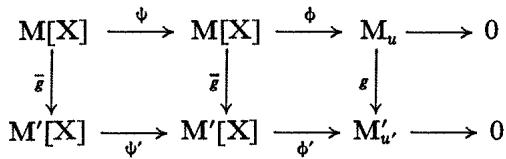
\includegraphics[keepaspectratio]{images/part004_f53e3a23.jpg}}

is commutative.

The condition \(g \circ u = u' \circ g\) is obviously necessary by (43) for \(g\) to be an A{[}X{]}-homomorphism; it is sufficient, for it implies by induction that \(g \circ u^n = u'^n \circ g\) for every integer \(n > 0\) . On the other hand, for all \(x \in M\) and all \(p \in A[X]\) ,

\[
\phi^ {\prime} (\bar {g} (p \otimes x)) = \phi^ {\prime} (p \otimes g (x)) = p (u ^ {\prime}) (g (x)) = g (p (u) (x)) = g (\phi (p \otimes x))
\]

and

\[
\bar {u} ^ {\prime} (\bar {g} (\boldsymbol {p} \otimes x)) = \bar {u} ^ {\prime} (\boldsymbol {p} \otimes g (x)) = \boldsymbol {p} \otimes u ^ {\prime} (g (x)) = \boldsymbol {p} \otimes g (u (x)) = \bar {g} (\bar {u} (\boldsymbol {p} \otimes x))
\]

which proves the commutativity of diagram (48).

\subsection{CHARACTERISTIC POLYNOMIAL OF AN ENDOMORPHISM}

Let M be a free A-module of dimension n and u an endomorphism of M. Consider the polynomial ring in two indeterminates A{[}X, Y{]} and the A{[}X, Y{]}-module M{[}X, Y{]} = A{[}X, Y{]} ⊗\_A M; let \(\bar{u}\) be the endomorphism of the A{[}X, Y{]}-module M{[}X, Y{]} canonically derived from u (II, §5, no. 1). It follows from no. 5, Proposition 11 that

\[
\det (\mathbf {X} - \mathbf {Y} \bar {\boldsymbol {u}}) = \sum_ {j = 0} ^ {n} (- 1) ^ {j} \operatorname{Tr} \left(\bigwedge^ {j} (u)\right) \mathbf {X} ^ {n - j} \mathbf {Y} ^ {j}\tag{49}
\]

for if \(U\) is the matrix of \(u\) with respect to a basis \((e_i)_{1 \leqslant i \leqslant n}\) of \(\mathbf{M}\) , \(U\) is the matrix of \(\bar{u}\) with respect to the basis \((1 \otimes e_i)_{1 \leqslant i \leqslant n}\) of \(\mathbf{M}[\mathbf{X}, \mathbf{Y}]\) , hence

\[
\operatorname{Tr} \left(\bigwedge^ {j} (\bar {u})\right) = \operatorname{Tr} \left(\bigwedge^ {j} (u)\right).
\]

DEFINITION 3. Let M be a finite-dimensional free A-module and u an endomorphism of M. The determinant of the endomorphism X - \(\bar{u}\) of the free A{[}X{]}-module M{[}X{]} is called the characteristic polynomial of u and is denoted by \(\chi_u(X)\) .

If \(\mathbf{M}\) is of rank \(n\) , it follows from (49) that

\[
\chi_ {u} (\mathbf {X}) = \sum_ {j = 0} ^ {n} (- 1) ^ {j} \operatorname{Tr} \left(\bigwedge^ {j} (u)\right) \mathbf {X} ^ {n - j}\tag{50}
\]

for \(\operatorname{det}(\mathbf{X} - \mathbf{Y}\bar{u}) = \operatorname{det}(\mathbf{X}.I_n + \mathbf{Y}U)\) and \(\operatorname{det}(\mathbf{X} - \bar{u}) = \operatorname{det}(\mathbf{X}.I_n - U)\) . It is therefore seen that \(\chi_u(\mathbf{X})\) is a monic polynomial of degree \(n\) , in which the coefficient of \(\mathbf{X}^{n-1}\) is \(-\mathrm{Tr}(u)\) and the constant term is \((-1)^n \operatorname{det}(u)\) .

PROPOSITION 20 (``Cayley-Hamilton theorem''). For every endomorphism \(u\) of a finite-dimensional free A-module, \(\chi_u(u) = 0\) .

In the notation of Proposition 18 (§ 3, no. 10), for all \(x \in \mathbf{M}\) , \(\chi_u(u)(x)\) is the image under \(\phi\) of \(\chi_u(\mathbf{X}) \otimes x\) . But if \(v\) is the endomorphism of \(\mathbf{M}[\mathbf{X}]\) , the co-transpose of \(\mathbf{X} - \bar{u}\) (no. 6), then

\[
\chi_ {u} (\mathbf {X}) \otimes x = \chi_ {u} (\mathbf {X}) (1 \otimes x) = (\mathbf {X} - \bar {u}) (v (1 \otimes x))
\]

and the conclusion follows from Proposition 18 of no. 10.

\section{NORMS AND TRACES}

Throughout this paragraph, K will denote a commutative ring and A a unital associative K-algebra. Every A-module will be assumed to be given the K-module structure obtained by restricting the scalars to K.
